
%DIF LATEXDIFF DIFFERENCE FILE
%DIF DEL main_1.tex   Sat Sep 26 09:49:11 2026
%DIF ADD main.tex     Sat Sep 26 09:48:43 2026
%% ============================================================================
%%  It Is Not the Signature: A Discarded Key-Parse Attempt Dominates Token
%%  Validation Cost in a Node.js Service
%%
%%  Submission build for a Springer Nature journal (sn-jnl.cls, sn-basic,
%%  two-column, numeric citations).
%%
%%  EVERY numeric value in the body is a macro from keypath_macros.tex, which
%DIF 10-12c10-16
%DIF < %%  the replication package generates from files under data/runs/ and survey/.
%DIF < %%  No digit is typed below. keypath_macros_provenance.csv maps each macro to
%DIF < %%  the file it was read from.
%DIF -------
%%  the replication package generates from files under data/runs/ and survey/, %DIF > 
%%  or from revision_macros.tex (analysis/make_revision_macros.py), which holds %DIF > 
%%  the measurements added in the 2026-09-24 revision: the plain-C OpenSSL %DIF > 
%%  probe, the V8 exception baseline, the x86_64 repetition of Tables 1-2 and %DIF > 
%%  the cross-library comparison. No digit is typed below. %DIF > 
%%  keypath_macros_provenance.csv and revision_macros_provenance.csv map each %DIF > 
%%  macro to the file it was read from. %DIF > 
%DIF -------
%%
%DIF 14c18-21
%DIF < %%  Figures are built from committed CSVs by figures/make_figures.py.
%DIF -------
%%  REVISION 2026-09-24 (base: main_1.tex). See CHANGES.md for every edit. %DIF > 
%% %DIF > 
%%  Figures are built from committed data by %DIF > 
%%  figures/make_revision_standin_figures.py. %DIF > 
%DIF -------
%%
%%  BUILD
%%      latexmk -pdf main.tex          (or: pdflatex, bibtex, pdflatex x2)
%%
%%  If sn-jnl.cls is not installed, this file falls back to `article` plus
%%  sn-fallback.tex so the archive still compiles. See README.md.
%% ============================================================================

\IfFileExists{sn-jnl.cls}{%
  \documentclass[pdflatex,sn-basic,twocolumn]{sn-jnl}%
  \newcommand{\SNJNL}{}%
}{%
  \documentclass[10pt,twocolumn,a4paper]{article}%
}

%DIF 30a37-49
%% --------------------------------------------------------------------------- %DIF > 
%%  Page area. In two-column mode sn-jnl sets a 160 x 216 mm text block 26 mm %DIF > 
%%  from the top of an A4 page, which leaves about 55 mm empty at the foot of %DIF > 
%%  every page. \fillpagetrue enlarges the text block so pages are used fully. %DIF > 
%%  Springer re-typesets accepted papers in its own layout, so this only affects %DIF > 
%%  the submission PDF. Set \fillpagefalse to restore the template exactly. %DIF > 
%% --------------------------------------------------------------------------- %DIF > 
\newif\iffillpage %DIF > 
\fillpagetrue %DIF > 
\ifdefined\SNJNL\iffillpage %DIF > 
  \geometry{top=20mm,text={170mm,250mm},headsep=4mm,footskip=8mm,bindingoffset=0mm} %DIF > 
\fi\fi %DIF > 
 %DIF > 
%DIF -------
\IfFileExists{lmodern.sty}{\usepackage{lmodern}}{} % optional; present on Overleaf
\usepackage{amsmath}
\usepackage{amssymb}
\usepackage{graphicx}
\usepackage{booktabs}
\usepackage{url}
\usepackage{xcolor}
\usepackage{listings}
%DIF 38a58-60
% sn-jnl.cls declares its footnote set with manyfoot at \begin{document}; %DIF > 
% main_1.tex no longer loaded it, which stops the build under the class. %DIF > 
\ifdefined\SNJNL\usepackage{manyfoot}\fi %DIF > 
%DIF -------

\ifdefined\SNJNL\else%% sn-fallback.tex -- minimal stand-ins for the sn-jnl.cls commands main.tex
%% uses, so the manuscript still compiles under `article` when the Springer
%% class is unavailable. Layout is not the journal's; content is identical.
%% (Stand-in written in the 2026-09-24 revision; replace with your own copy if
%% you have one.)
\usepackage{hyperref}
\makeatletter
\def\title{\@ifnextchar[{\sn@title}{\sn@title[]}}
\def\sn@title[#1]#2{\gdef\@title{#2}}
\newcommand{\fnm}[1]{#1}
\newcommand{\sur}[1]{#1}
\newcommand{\email}[1]{}
\let\sn@author\author
\gdef\sn@authors{}
\renewcommand{\author}{\@ifstar{\sn@auth}{\sn@auth}}
\newcommand{\sn@auth}[2][]{\g@addto@macro\sn@authors{\and #2\textsuperscript{#1}}}
\newcommand{\affil}[2][]{}
\newcommand{\orgdiv}[1]{#1}\newcommand{\orgname}[1]{#1}
\newcommand{\city}[1]{#1}\newcommand{\state}[1]{#1}\newcommand{\country}[1]{#1}
\long\def\abstract#1{\gdef\sn@abstract{#1}}
\newcommand{\keywords}[1]{\gdef\sn@keywords{#1}}
\let\sn@maketitle\maketitle
\renewcommand{\maketitle}{%
  \expandafter\sn@author\expandafter{\sn@authors}%
  \twocolumn[{\sn@maketitle\begin{quote}\small\textbf{Abstract.} \sn@abstract
  \par\medskip\textbf{Keywords:} \sn@keywords\end{quote}\medskip}]}
\newcommand{\backmatter}{}
\newcommand{\bmhead}[1]{\paragraph{#1}}
\makeatother
\fi

\graphicspath{{figures/}}

\input{keypath_macros}
%DIF 44a67
\input{revision_macros}   % revision items 6, 7, 8, 10 %DIF > 
%DIF -------

%DIF 45-87c69-71
%DIF < %% ---------------------------------------------------------------------------
%DIF < %%  A/B corroboration macros (Section~\ref{sec:abcorroboration}).
%DIF < %%
%DIF < %%  ALIAS BLOCK — edit ONLY this, then delete it once the names match.
%DIF < %%  make_keypath_macros.py emits its own A/B names; map them on with \let, e.g.
%DIF < %%
%DIF < %%      \let\ABEnabledMean\AbValidationOnMeanUs
%DIF < %%
%DIF < %%  or rename in the generator and drop this block. The \providecommand lines
%DIF < %%  render "??" so an unmapped macro cannot be shipped by accident.
%DIF < %% ---------------------------------------------------------------------------
%DIF < \providecommand{\ABRunId}{??}          % run directory, e.g. INSITU-2026-09-14-ab
%DIF < \providecommand{\ABRate}{??}           % arrival rate, requests/s
%DIF < \providecommand{\ABWindowSeconds}{??}  % window duration, seconds
%DIF < \providecommand{\ABEnabledMean}{??}    % per-call mean, validation enabled (us)
%DIF < \providecommand{\ABDisabledMean}{??}   % per-call mean, validation disabled (us)
%DIF < \providecommand{\ABEnabledCalls}{??}   % histogram _count delta, enabled
%DIF < \providecommand{\ABDisabledCalls}{??}  % histogram _count delta, disabled
%DIF < \providecommand{\ABEnabledLoad}{??}    % 1-min load average at window start
%DIF < \providecommand{\ABDisabledLoad}{??}   % 1-min load average at window start
%DIF < \providecommand{\ABDelta}{??}          % enabled minus disabled (us)
%DIF < \providecommand{\ABDeltaPct}{??}       % delta as a share of the enabled mean
%DIF < \providecommand{\ABQuantity}{per-request handler time}  % what the means time
%DIF < 
%DIF < %% GUARD. If any A/B macro is still the literal "??", Section 6.4 falls back to
%DIF < %% a version that reports no numbers, and the build prints a warning. It is
%DIF < %% therefore impossible to submit a PDF containing "??" in Table 4.
%DIF < %% Once the alias block above is mapped, this flips itself and the full
%DIF < %% subsection with Table 4 is typeset. No manual switch to remember.
%DIF < \newif\ifabdata \abdatatrue
%DIF < \makeatletter
%DIF < \newcommand{\ab@unset}{??}  % \newcommand, not \def: both must be \long for \ifx
%DIF < \newcommand{\ab@check}[1]{\ifx#1\ab@unset\global\abdatafalse\fi}
%DIF < \ab@check\ABRunId        \ab@check\ABRate          \ab@check\ABWindowSeconds
%DIF < \ab@check\ABEnabledMean  \ab@check\ABDisabledMean  \ab@check\ABEnabledCalls
%DIF < \ab@check\ABDisabledCalls\ab@check\ABEnabledLoad   \ab@check\ABDisabledLoad
%DIF < \ab@check\ABDelta        \ab@check\ABDeltaPct
%DIF < \ifabdata\else
%DIF <   \AtBeginDocument{\typeout{^^J*** A/B data not mapped: Section 6.4 is in its
%DIF <   no-numbers form and Table 4 is omitted. Map the \string\AB... alias block
%DIF <   to restore it. ***^^J}}
%DIF < \fi
%DIF < \makeatother
%DIF -------
%% A/B corroboration (Section~\ref{sec:abcorroboration}) reads the cgroup CPU %DIF > 
%% macros \Ab... that make_keypath_macros.py emits; the earlier \AB... alias %DIF > 
%% block and its no-numbers fallback are no longer needed and were removed. %DIF > 
%DIF -------

%% ---------------------------------------------------------------------------
%%  Author-facing placeholders.
%%
%%  Seven facts are known only to the authors and are marked below. While
%%  \showauthornotestrue they are typeset in red so they cannot be missed;
%%  set \showauthornotesfalse for a clean preview. Replace each one and then
%%  delete this block together with the \TODO and \AUTHORNOTE macros.
%% ---------------------------------------------------------------------------
\definecolor{notered}{HTML}{B02A1E}
\newif\ifshowauthornotes
\showauthornotestrue            % <-- set to \showauthornotesfalse to hide

% Inline placeholder: always typesets, highlighted while notes are shown.
\newcommand{\TODO}[1]{\ifshowauthornotes\textcolor{notered}{\textbf{#1}}\else#1\fi}
% Standalone editorial note: vanishes entirely when notes are hidden.
\newcommand{\AUTHORNOTE}[1]{\ifshowauthornotes
  \par\begingroup\color{notered}\footnotesize\noindent
  \textbf{[AUTHORS]\ }#1\par\endgroup\fi}

\newcommand{\LibraryName}{\texttt{jsonwebtoken}}
%DIF 109-111c93-100
%DIF < \newcommand{\LibraryVersion}{\TODO{version~9.0.3}}
%DIF < \newcommand{\LibraryTag}{\TODO{tag~v9.0.3}}
%DIF < \newcommand{\CodeFileLines}{\TODO{verify.js, lines 99--110}}
%DIF -------
%% Confirmed 2026-09-24: bench/node_modules/jsonwebtoken/verify.js (the file %DIF > 
%% measured) is byte-identical to verify.js at tag v9.0.3, commit ed59e76, %DIF > 
%% sha256 fa01db296dfa5585bff7b097187ef65fcb017d636ab9900799eb53e0acee0b85. %DIF > 
%% The key-resolution block is at lines 120--130 there; the earlier placeholder %DIF > 
%% (99--110) was taken from master and was wrong for the release. %DIF > 
\newcommand{\LibraryVersion}{version~9.0.3} %DIF > 
\newcommand{\LibraryTag}{tag~v9.0.3} %DIF > 
\newcommand{\CodeFileLines}{verify.js, lines 120--130} %DIF > 
%DIF -------
%% CodeFirstLine must be a bare integer (listings uses it arithmetically).
%% The four macros above are produced by make_codepath_figure.py from the
%% pinned release; run it and \input the file it writes, which overrides them:
%%     python3 make_codepath_figure.py path/to/node_modules/jsonwebtoken
%%     \input{figures/codepath_macros}
%DIF 117-119c106-110
%DIF < %% The values below are placeholders taken from the package's master branch and
%DIF < %% MUST be confirmed against the release you actually measured.
%DIF < \newcommand{\CodeFirstLine}{99}
%DIF -------
%% Confirmed against v9.0.3: figures/codepath_excerpt.js is lines 120--130 of %DIF > 
%% verify.js with four spaces of common indentation removed; its full sha256 is %DIF > 
%% 4c4781826f49fa9006cb8e42be400c46953870c7d46f4219ec342330ba8ced71, whose %DIF > 
%% prefix is the value below. %DIF > 
\newcommand{\CodeFirstLine}{120} %DIF > 
%DIF -------
\newcommand{\CodeExcerptHash}{sha256:4c4781826f49fa90}
%DIF 121c112-115
%DIF < \newcommand{\NaiveFailingTests}{\TODO{both in \texttt{test/wrong\_alg.tests.js}; insert the two \texttt{it()} titles from the failing run}}
%DIF -------
%% Read from data/runs/2026-09-24-upstream-suite-x86_64/unrestricted.txt. %DIF > 
\newcommand{\NaiveFailingTests}{``should not allow HMAC verification with an RSA %DIF > 
key in PEM format'' and, under ``signing with pub key as symmetric'', ``should %DIF > 
not verify''} %DIF > 
%DIF -------

%% ---------------------------------------------------------------------------
\lstdefinelanguage{JavaScriptX}{
  keywords={typeof, new, true, false, catch, function, return, null, switch,
            var, if, in, while, do, else, case, break, const, let, try, throw},
  ndkeywords={class, export, import, this, require, module},
  sensitive=true,
  comment=[l]{//},
  morecomment=[s]{/*}{*/},
  morestring=[b]',
  morestring=[b]"
}
\lstset{
  language=JavaScriptX,
  basicstyle=\ttfamily\scriptsize,
  keywordstyle=\bfseries,
  commentstyle=\itshape\color[HTML]{52514E},
  stringstyle=\color[HTML]{1B6E4A},
  numbers=left,
  numberstyle=\tiny\color[HTML]{8A8984},
  numbersep=5pt,
  breaklines=true,
  frame=single,
  rulecolor=\color[HTML]{C9C8C3},
  framesep=4pt,
  columns=fullflexible,
  keepspaces=true,
  showstringspaces=false,
  xleftmargin=2pt,
  aboveskip=4pt,
  belowskip=2pt,
}

\IfFileExists{microtype.sty}{\usepackage{microtype}}{}
\emergencystretch=3em
\hyphenation{
  micro-ser-vices micro-ser-vice micro-bench-mark micro-bench-marks
  cryp-to-graph-ic cryp-tog-ra-phy au-then-ti-ca-tion va-li-da-tion
  in-stru-men-ta-tion con-fig-u-ra-tion im-ple-men-ta-tion
  Ku-ber-netes side-car side-cars name-space through-put
  pre-parsed re-pro-duc-i-ble de-ploy-ment mea-sure-ment
}
%DIF < \raggedbottom
%DIF -------
%% --------------------------------------------------------------------------- %DIF > 
%%  Page filling. LaTeX's default float limits (at most 70% of a page, at most %DIF > 
%%  two floats at the top) push floats to later pages and leave columns short; %DIF > 
%%  with \raggedbottom that showed as blank space at the foot of many pages. %DIF > 
%%  These values let floats sit where they are first referenced and make both %DIF > 
%%  columns end at the same height. %DIF > 
%% --------------------------------------------------------------------------- %DIF > 
\renewcommand{\topfraction}{0.9} %DIF > 
\renewcommand{\bottomfraction}{0.8} %DIF > 
\renewcommand{\textfraction}{0.07} %DIF > 
\renewcommand{\floatpagefraction}{0.85} %DIF > 
\renewcommand{\dbltopfraction}{0.9} %DIF > 
\renewcommand{\dblfloatpagefraction}{0.85} %DIF > 
\setcounter{topnumber}{4} %DIF > 
\setcounter{bottomnumber}{3} %DIF > 
\setcounter{totalnumber}{6} %DIF > 
\setcounter{dbltopnumber}{3} %DIF > 
\setlength{\floatsep}{8pt plus 2pt minus 2pt} %DIF > 
\setlength{\textfloatsep}{10pt plus 2pt minus 3pt} %DIF > 
\setlength{\intextsep}{8pt plus 2pt minus 2pt} %DIF > 
\setlength{\dblfloatsep}{8pt plus 2pt minus 2pt} %DIF > 
\setlength{\dbltextfloatsep}{10pt plus 2pt minus 3pt} %DIF > 
\flushbottom %DIF > 
%% A little vertical stretch between paragraphs so \flushbottom can fill a %DIF > 
%% column without leaving the slack at its foot. %DIF > 
\AtBeginDocument{\setlength{\parskip}{0pt plus 1.5pt}} %DIF > 
%DIF PREAMBLE EXTENSION ADDED BY LATEXDIFF
%DIF UNDERLINE PREAMBLE %DIF PREAMBLE
\RequirePackage[normalem]{ulem} %DIF PREAMBLE
\RequirePackage{color}\definecolor{RED}{rgb}{1,0,0}\definecolor{BLUE}{rgb}{0,0,1} %DIF PREAMBLE
\providecommand{\DIFadd}[1]{{\protect\color{blue}\uwave{#1}}} %DIF PREAMBLE
\providecommand{\DIFdel}[1]{{\protect\color{red}\sout{#1}}}                      %DIF PREAMBLE
%DIF SAFE PREAMBLE %DIF PREAMBLE
\providecommand{\DIFaddbegin}{} %DIF PREAMBLE
\providecommand{\DIFaddend}{} %DIF PREAMBLE
\providecommand{\DIFdelbegin}{} %DIF PREAMBLE
\providecommand{\DIFdelend}{} %DIF PREAMBLE
\providecommand{\DIFmodbegin}{} %DIF PREAMBLE
\providecommand{\DIFmodend}{} %DIF PREAMBLE
%DIF FLOATSAFE PREAMBLE %DIF PREAMBLE
\providecommand{\DIFaddFL}[1]{\DIFadd{#1}} %DIF PREAMBLE
\providecommand{\DIFdelFL}[1]{\DIFdel{#1}} %DIF PREAMBLE
\providecommand{\DIFaddbeginFL}{} %DIF PREAMBLE
\providecommand{\DIFaddendFL}{} %DIF PREAMBLE
\providecommand{\DIFdelbeginFL}{} %DIF PREAMBLE
\providecommand{\DIFdelendFL}{} %DIF PREAMBLE
\newcommand{\DIFscaledelfig}{0.5}
%DIF HIGHLIGHTGRAPHICS PREAMBLE %DIF PREAMBLE
\RequirePackage{settobox} %DIF PREAMBLE
\RequirePackage{letltxmacro} %DIF PREAMBLE
\newsavebox{\DIFdelgraphicsbox} %DIF PREAMBLE
\newlength{\DIFdelgraphicswidth} %DIF PREAMBLE
\newlength{\DIFdelgraphicsheight} %DIF PREAMBLE
% store original definition of \includegraphics %DIF PREAMBLE
\LetLtxMacro{\DIFOincludegraphics}{\includegraphics} %DIF PREAMBLE
\newcommand{\DIFaddincludegraphics}[2][]{{\color{blue}\fbox{\DIFOincludegraphics[#1]{#2}}}} %DIF PREAMBLE
\newcommand{\DIFdelincludegraphics}[2][]{% %DIF PREAMBLE
\sbox{\DIFdelgraphicsbox}{\DIFOincludegraphics[#1]{#2}}% %DIF PREAMBLE
\settoboxwidth{\DIFdelgraphicswidth}{\DIFdelgraphicsbox} %DIF PREAMBLE
\settoboxtotalheight{\DIFdelgraphicsheight}{\DIFdelgraphicsbox} %DIF PREAMBLE
\scalebox{\DIFscaledelfig}{% %DIF PREAMBLE
\parbox[b]{\DIFdelgraphicswidth}{\usebox{\DIFdelgraphicsbox}\\[-\baselineskip] \rule{\DIFdelgraphicswidth}{0em}}\llap{\resizebox{\DIFdelgraphicswidth}{\DIFdelgraphicsheight}{% %DIF PREAMBLE
\setlength{\unitlength}{\DIFdelgraphicswidth}% %DIF PREAMBLE
\begin{picture}(1,1)% %DIF PREAMBLE
\thicklines\linethickness{2pt} %DIF PREAMBLE
{\color[rgb]{1,0,0}\put(0,0){\framebox(1,1){}}}% %DIF PREAMBLE
{\color[rgb]{1,0,0}\put(0,0){\line( 1,1){1}}}% %DIF PREAMBLE
{\color[rgb]{1,0,0}\put(0,1){\line(1,-1){1}}}% %DIF PREAMBLE
\end{picture}% %DIF PREAMBLE
}\hspace*{3pt}}} %DIF PREAMBLE
} %DIF PREAMBLE
\LetLtxMacro{\DIFOaddbegin}{\DIFaddbegin} %DIF PREAMBLE
\LetLtxMacro{\DIFOaddend}{\DIFaddend} %DIF PREAMBLE
\LetLtxMacro{\DIFOdelbegin}{\DIFdelbegin} %DIF PREAMBLE
\LetLtxMacro{\DIFOdelend}{\DIFdelend} %DIF PREAMBLE
\DeclareRobustCommand{\DIFaddbegin}{\DIFOaddbegin \let\includegraphics\DIFaddincludegraphics} %DIF PREAMBLE
\DeclareRobustCommand{\DIFaddend}{\DIFOaddend \let\includegraphics\DIFOincludegraphics} %DIF PREAMBLE
\DeclareRobustCommand{\DIFdelbegin}{\DIFOdelbegin \let\includegraphics\DIFdelincludegraphics} %DIF PREAMBLE
\DeclareRobustCommand{\DIFdelend}{\DIFOaddend \let\includegraphics\DIFOincludegraphics} %DIF PREAMBLE
\LetLtxMacro{\DIFOaddbeginFL}{\DIFaddbeginFL} %DIF PREAMBLE
\LetLtxMacro{\DIFOaddendFL}{\DIFaddendFL} %DIF PREAMBLE
\LetLtxMacro{\DIFOdelbeginFL}{\DIFdelbeginFL} %DIF PREAMBLE
\LetLtxMacro{\DIFOdelendFL}{\DIFdelendFL} %DIF PREAMBLE
\DeclareRobustCommand{\DIFaddbeginFL}{\DIFOaddbeginFL \let\includegraphics\DIFaddincludegraphics} %DIF PREAMBLE
\DeclareRobustCommand{\DIFaddendFL}{\DIFOaddendFL \let\includegraphics\DIFOincludegraphics} %DIF PREAMBLE
\DeclareRobustCommand{\DIFdelbeginFL}{\DIFOdelbeginFL \let\includegraphics\DIFdelincludegraphics} %DIF PREAMBLE
\DeclareRobustCommand{\DIFdelendFL}{\DIFOaddendFL \let\includegraphics\DIFOincludegraphics} %DIF PREAMBLE
%DIF COLORLISTINGS PREAMBLE %DIF PREAMBLE
\RequirePackage{listings} %DIF PREAMBLE
\RequirePackage{color} %DIF PREAMBLE
\lstdefinelanguage{DIFcode}{ %DIF PREAMBLE
%DIF DIFCODE_UNDERLINE %DIF PREAMBLE
  moredelim=[il][\color{red}\sout]{\%DIF\ <\ }, %DIF PREAMBLE
  moredelim=[il][\color{blue}\uwave]{\%DIF\ >\ } %DIF PREAMBLE
} %DIF PREAMBLE
\lstdefinestyle{DIFverbatimstyle}{ %DIF PREAMBLE
	language=DIFcode, %DIF PREAMBLE
	basicstyle=\ttfamily, %DIF PREAMBLE
	columns=fullflexible, %DIF PREAMBLE
	keepspaces=true %DIF PREAMBLE
} %DIF PREAMBLE
\lstnewenvironment{DIFverbatim}{\lstset{style=DIFverbatimstyle}}{} %DIF PREAMBLE
\lstnewenvironment{DIFverbatim*}{\lstset{style=DIFverbatimstyle,showspaces=true}}{} %DIF PREAMBLE
%DIF END PREAMBLE EXTENSION ADDED BY LATEXDIFF

\begin{document}

\title[It Is Not the Signature]{It Is Not the Signature: A Discarded Key-Parse
Attempt Dominates Token Validation Cost in a Node.js Service}

\author[1,3]{\fnm{Jannatul Ferdous} \sur{Katha}}\email{ferdous.katha@elitelab.ai}
\author[2,3]{\fnm{Tasmia Tahmid} \sur{Prova}}\email{tasmia.prova@elitelab.ai}
\author[3]{\fnm{Md Kishor} \sur{Morol}}\email{kishormorol@ieee.org}
\author*[4]{\fnm{Tze Hui} \sur{Liew}}\email{thliew@mmu.edu.my}
\author[3,5]{\fnm{Dip} \sur{Nandi}}\email{dip.nandi@aiub.edu}

\affil[1]{\orgdiv{Department of CSE}, \orgname{Bangladesh University of Professionals (BUP)}, \city{Dhaka}, \country{Bangladesh}}
\affil[2]{\orgdiv{Department of CSE}, \orgname{Bangladesh University of Business and Technology (BUBT)}, \city{Dhaka}, \country{Bangladesh}}
\affil[3]{\orgname{ELITE Research Lab}, \city{Queens}, \state{NY}, \country{USA}}
\affil[4]{\orgdiv{Faculty of Information Science and Technology}, \orgname{Multimedia University}, \city{Melaka}, \country{Malaysia}}
\affil[5]{\orgdiv{Department of Computer Science}, \orgname{American International University-Bangladesh (AIUB)}, \city{Dhaka}, \country{Bangladesh}}

\DIFdelbegin %DIFDELCMD < \abstract{The per-request cost of JSON Web Token validation is routinely
%DIFDELCMD < attributed to cryptography. We report that for a widely used Node.js library
%DIFDELCMD < the attribution is wrong, and that the natural repair --- moving the cost to key
%DIFDELCMD < conversion --- is wrong too. When a shared secret is supplied as a string, which
%DIFDELCMD < is what the
%DIFDELCMD < library's interface invites --- \LibraryName{} resolves it by attempting to
%DIFDELCMD < parse it as an \emph{asymmetric} key first, falling back to the symmetric
%DIFDELCMD < constructor only after that attempt throws. The conversion it falls back to
%DIFDELCMD < costs \HostCreateSecretKey~$\mu$s and explains nothing. The discarded attempt
%DIFDELCMD < preceding it costs \HostProbeThrows~$\mu$s, \HostProbeShareOfCall\% of the call
%DIFDELCMD < and its largest single component. Two independent methods agree: differencing
%DIFDELCMD < timed conditions across \HostInvocations{} separate processes, and a sampling
%DIFDELCMD < profiler attributing a median \ProfHostPct\% of self time to that parse. We do
%DIFDELCMD < not separate the cost of the parse attempt from the cost of constructing and
%DIFDELCMD < discarding the exception that ends it; the two are reported as one component
%DIFDELCMD < and every claim is stated at that granularity. Holding containerisation
%DIFDELCMD < constant and varying the runtime, the magnitude co-varies with the bundled
%DIFDELCMD < OpenSSL version across four images, spanning \SpanProbeThrows$\times$; two
%DIFDELCMD < major engine versions sharing one OpenSSL series do not differ, but the design
%DIFDELCMD < cannot separate the faster OpenSSL from the newer engine shipped alongside it,
%DIFDELCMD < so we state a co-variation rather than a cause. The cost persists in a deployed
%DIFDELCMD < service, measured across seven arrival rates. The avoiding pattern is rare
%DIFDELCMD < \emph{in our sample}: \SampleSitesPreparsed{} of \SampleCallSites{} classified
%DIFDELCMD < call sites across \SampleRepos{} repositories pass a pre-parsed key, and among
%DIFDELCMD < \CounterReposWithVerify{} repositories that both reference the pre-parsing
%DIFDELCMD < interface and call the validator, \AdjudicatedGenuineProjects{} use it. These
%DIFDELCMD < are samples with unknown inclusion probabilities and no population proportion
%DIFDELCMD < follows from them. We propose a fix, and report a constraint on it we consider
%DIFDELCMD < the more important result: the discarded attempt is load-bearing for an
%DIFDELCMD < existing key-type defence, so the obvious form of the optimisation must not be
%DIFDELCMD < applied. All measurements come from one ARM64 host.}
%DIFDELCMD < %%%
\DIFdelend \DIFaddbegin \abstract{A performance cost is only as well attributed as the components
recorded alongside it. We show this for JSON Web Token validation, whose
per-request cost is routinely attributed to cryptography. In
\LibraryName{}, the widely used Node.js library, the signature primitive is
\HostHmacString~$\mu$s of a \HostJwtString~$\mu$s call. The dominant component,
\HostProbeThrows~$\mu$s or \HostProbeShareOfCall\%, is a discarded parse: given a
shared secret as a string, the library first tries to parse it as an
asymmetric key and falls back only after that attempt fails. Differencing
across \HostInvocations{} processes and a sampling profiler agree on this. Its
price is set by the OpenSSL release a runtime bundles, and the evidence is
causal. The same OpenSSL calls issued from C, against \CProbeVersionCount{}
identically built releases, cost \CFullVThreeZeroSixteen~$\mu$s on
\CVersionLiteralVThreeZeroSixteen{} and \CFullVThreeFiveEight~$\mu$s on
\CVersionLiteralVThreeFiveEight. A newer JavaScript engine paired with an older
OpenSSL is the slow runtime, and the exception V8 builds costs a few
microseconds. In deployment, validation adds \AbCpuPerCallDelta~$\mu$s of
processor time per request, within \AbCpuVsPredictedPct\% of the
microbenchmark prediction. Of seven JWT libraries in four languages, only this
one attempts the parse; five pay nothing for a raw secret. The avoiding pattern
is rare in public code, and the obvious fix would disable a key-type defence
that the discarded parse makes possible; we give a narrow fix that preserves
it and have reported the defect upstream.}
\DIFaddend 

\keywords{JSON Web Token, JWT, key resolution, performance measurement,
benchmarking methodology, Node.js, OpenSSL 3.x, software defect}

\maketitle

%% ============================================================================
\section{Introduction}\label{sec:intro}

Authentication in cloud-native services is commonly described as imposing a
per-request cryptographic cost~\DIFdelbegin %DIFDELCMD < \cite{zhu2023dissecting}%%%
\DIFdelend \DIFaddbegin \citep{zhu2023dissecting}\DIFaddend .
The assumption is old and has been tested before, one layer down: \DIFdelbegin \DIFdel{Coarfa et
al.~}%DIFDELCMD < \cite{coarfa2006performance} %%%
\DIFdelend \DIFaddbegin \citet{coarfa2006performance} \DIFaddend instrumented TLS web servers and found RSA
responsible for only a minority of server cost, the remainder falling to
symmetric operations, hashing and protocol handling. Our result is that
argument repeated at the application layer, and reaching a sharper version of
the same conclusion.

The reasoning being tested is intuitive: validating a JSON Web
Token~\DIFdelbegin %DIFDELCMD < \cite{rfc7519} %%%
\DIFdelend \DIFaddbegin \citep{rfc7519} \DIFaddend means verifying a signature, signatures are cryptography,
and cryptography is expensive relative to parsing. The conclusion usually drawn
is that the cost should be \emph{moved} --- to a sidecar proxy, a gateway, or
dedicated hardware --- because specialised components do cryptographic work
well.

We report that the premise is wrong for the most widely used JavaScript
implementation we could measure. The natural repair is wrong as well. Once the
signature primitive is shown to be a small share of the cost, the remainder is
readily attributed to key material being converted from a string into a key
object on every call. Measuring that conversion directly puts it at
\HostCreateSecretKey~$\mu$s: too small to be the explanation for anything.

The actual mechanism is a control-flow accident, shown in
Figure~\ref{fig:codepath}. Given a secret that is not already a key object, the
library attempts \texttt{createPublicKey()} first and falls back to
\texttt{createSecretKey()} in the exception handler. For an HMAC secret the
first call cannot succeed. Every validation therefore constructs and discards
an OpenSSL parse failure, at \HostProbeThrows~$\mu$s against a total call cost
of \HostJwtString~$\mu$s.

We are careful about what that \HostProbeThrows~$\mu$s is. It is the cost of
the whole discarded attempt: the work OpenSSL performs before deciding the
input is not an asymmetric key, plus the construction and unwinding of the
exception that carries that decision back to the library.
\DIFdelbegin \DIFdel{We measure the pair.
We do not separate them, and }\DIFdelend Section~\ref{sec:granularity} \DIFdelbegin \DIFdel{states the bound our
data does place on the split. The paper's title and claims are pitched at the granularity we measured.
}\DIFdelend \DIFaddbegin \DIFadd{separates the two, by reissuing the OpenSSL calls
from C and by measuring an exception of the same shape with no OpenSSL call.
Where the attempt is expensive it is almost all parse; the exception is a few
microseconds. The title's ``key-parse attempt'' is therefore the accurate
name, and ``discarded exception'' would not be.
}\DIFaddend 

\paragraph{Research questions}
\DIFdelbegin %DIFDELCMD < \begin{description}
\begin{description}%DIFAUXCMD
%DIFDELCMD < \item[RQ1] %%%
\item[\DIFdel{RQ1}]%DIFAUXCMD
\DIFdel{Where does the per-request cost of token validation actually go?
}%DIFDELCMD < \item[RQ2] %%%
\item[\DIFdel{RQ2}]%DIFAUXCMD
\DIFdel{What does the magnitude of that cost co-vary with?
}%DIFDELCMD < \item[RQ3] %%%
\item[\DIFdel{RQ3}]%DIFAUXCMD
\DIFdel{Does it matter in a deployed service, and how common is the pattern
           that avoids it?
}
\end{description}%DIFAUXCMD
%DIFDELCMD < \end{description}
%DIFDELCMD < %%%
\DIFdelend \DIFaddbegin \begin{list}{}{\setlength{\labelwidth}{2.2em}\setlength{\labelsep}{0.5em}%
  \setlength{\leftmargin}{2.7em}\setlength{\itemsep}{1pt}\setlength{\topsep}{2pt}%
  \setlength{\parsep}{0pt}\renewcommand{\makelabel}[1]{\textbf{#1}\hfill}}
\item[\DIFadd{RQ1}] Where does the per-request cost of token validation actually go?
\item[\DIFadd{RQ2}] What governs the magnitude of that cost?
\item[\DIFadd{RQ3}] Does it matter in a deployed service, and how common is the
  pattern that avoids it?
\item[\DIFadd{RQ4}] Is the defect a property of one library, or of a design choice
  other libraries could share?
\end{list}
\DIFaddend 

\paragraph{Contributions} All supported by measurements in the replication
package~\DIFdelbegin %DIFDELCMD < \cite{artifact2026}%%%
\DIFdelend \DIFaddbegin \citep{artifact2026}\DIFaddend .

\begin{enumerate}
\item A decomposition of the validation call, by two independent methods,
      locating its dominant component in a discarded key-parse attempt rather
      than in the signature primitive or in key conversion\DIFaddbegin \DIFadd{, and a second
      decomposition of that attempt into the OpenSSL parse, the V8 exception
      and the binding between them }\DIFaddend (Section~\ref{sec:rq1}).
\item \DIFdelbegin \DIFdel{Evidence that the magnitude co-varies with the runtime's bundled OpenSSL version rather than with containerisation, together with an explicit
      statement of what the available runtime pairs cannot separate
      }\DIFdelend \DIFaddbegin \DIFadd{A causal attribution of its magnitude to the bundled OpenSSL release: the
      parse reissued from C with no JavaScript engine across
      }\CProbeVersionCount{} \DIFadd{identically built OpenSSL releases, a runtime pair
      that crosses engine and library, and a repetition on a second
      architecture }\DIFaddend (Section~\ref{sec:rq2}).
\item A deployed-service measurement across seven arrival rates, and a survey
      establishing that the avoiding pattern is rare in three samples of public
      code (Section~\ref{sec:rq3}).
\item A \DIFdelbegin \DIFdel{fix, and }\DIFdelend \DIFaddbegin \DIFadd{comparison of seven JWT libraries in four languages showing that the
      cost follows a design choice --- resolving key material on every call,
      of which a failing asymmetric parse used as a type test is the costliest
      form --- rather than JWT validation as such (Section~\ref{sec:rq4}).
}\item \DIFadd{A fix, }\DIFaddend a constraint on it\DIFaddbegin \DIFadd{, and an upstream report}\DIFaddend : the discarded attempt
      is load-bearing for an existing key-type defence, so the natural form of
      the optimisation is unsafe (Section~\ref{sec:fix}).
\end{enumerate}

%% ============================================================================
\section{Background and related work}\label{sec:related}

\paragraph{What a validation call does.} A JSON Web Token carries a header, a
payload and a signature over the first two~\DIFdelbegin %DIFDELCMD < \cite{rfc7519}%%%
\DIFdelend \DIFaddbegin \citep{rfc7519}\DIFaddend . Validating one means
decoding two segments, resolving key material into a form the cryptographic
library accepts, and verifying the signature. The middle step --- key
resolution --- is the subject of this paper, and it is the step most often left
implicit when validation cost is discussed.

\paragraph{Where the cost is usually attributed.} Published measurement of
layered enforcement in microservices concentrates on transport and proxy
layers. \DIFdelbegin \DIFdel{Zhu et al.~}%DIFDELCMD < \cite{zhu2023dissecting} %%%
\DIFdelend \DIFaddbegin \citet{zhu2023dissecting} \DIFaddend decompose service-mesh sidecar
overhead and show that the dominant contributors depend on configuration and
workload rather than being a fixed tax; we reach an analogous conclusion one
layer up, for application-level validation. Application-level token validation
is itself thinly evidenced, and is commonly reported as a difference between
scenario averages, which attributes to validation every difference between two
runs. We were unable to locate a study that measures the key-resolution step
directly;
we state that as an absence we searched for rather than as a claim about the
whole literature.

\paragraph{Cryptographic cost has been over-attributed before.} \DIFdelbegin \DIFdel{Coarfa et
al.~}%DIFDELCMD < \cite{coarfa2006performance} %%%
\DIFdelend \DIFaddbegin \citet{coarfa2006performance} \DIFaddend remains the clearest precedent: measuring TLS
web servers rather than primitives, they found the public-key operation was a
minority of server cost. Work on cryptographic library performance since has
largely stayed at the level of the primitive or the protocol
exchange~\DIFdelbegin %DIFDELCMD < \cite{naser2020performance,sikeridis2020assessing}%%%
\DIFdel{, with Tuveri and
Brumley~}%DIFDELCMD < \cite{tuveri2019engines} %%%
\DIFdelend \DIFaddbegin \citep{naser2020performance,sikeridis2020assessing}\DIFadd{, with }\citet{tuveri2019engines} \DIFaddend a notable exception in examining how a library
loads and dispatches implementations rather than how fast those
implementations run. Our result concerns neither: it is the cost of getting key
material \emph{into} the library.

\DIFaddbegin \paragraph{Performance bugs as a class.} \citet{jin2012understanding} \DIFadd{studied real-world performance bugs across five
code bases and found that most follow a small number of recurring patterns ---
among them uncoordinated and skippable function calls --- and that fixes are
usually local. }\citet{zaman2012qualitative} \DIFadd{found, from 400
Firefox and Chrome reports, that performance bugs differ from other bugs in
how they are reported, discussed and fixed, in part because reproducing them
is hard; }\citet{nistor2013discovering} \DIFadd{report that most are found
by code reasoning rather than by observing symptoms. }\citet{liu2014characterizing} \DIFadd{reach similar conclusions for mobile
applications. Detection work targets structural symptoms: redundant traversals
with similar memory-access patterns~}\citep{nistor2013toddler}\DIFadd{, or predicates
that separate slow from fast runs~}\citep{song2014statistical}\DIFadd{. The defect here
is of the ``skippable call'' kind Jin et al.\ describe, but it has none of the
structural signatures those detectors look for: it is one call, executed once
per request, whose failure is its only observable effect. It is also the shape
that makes a performance bug hard to report: our own upstream report was
preceded by a two-year-old report of the symptom with no diagnosed cause
(Section~\ref{sec:fix}).
}

\paragraph{JavaScript and Node.js performance.} \citet{selakovic2016performance} \DIFadd{classified performance issues in
JavaScript projects and found that inefficient API usage --- correct calls made
in a costly way --- is among the most common root causes, and that the fixes
are typically a few lines. Their later profiler~}\citep{selakovic2017actionable}
\DIFadd{targets precisely the }\emph{\DIFadd{order}} \DIFadd{in which a program evaluates conditions, the
axis on which this defect lives: a check that almost always fails is evaluated
before one that almost always succeeds. }\citet{gong2015jitprof}
\DIFadd{locate code that defeats JIT optimisation; exception-heavy control flow is one
such pattern, and Section~\ref{sec:granularity} measures what it costs here.
Work on the Node.js event loop shows why a per-request synchronous cost matters
beyond its magnitude: a single slow handler delays every other
client~}\citep{davis2018sense,staicu2018freezing}\DIFadd{. We make no availability or
capacity claim, but the mechanism by which a synchronous per-request cost
propagates is the same.
}

\DIFaddend \paragraph{Version and environment variation.} That software performance
changes across versions in ways maintainers do not anticipate is established:
\DIFdelbegin \DIFdel{Kaltenecker et al.~}%DIFDELCMD < \cite{kaltenecker2023performance} %%%
\DIFdelend \DIFaddbegin \citet{kaltenecker2023performance} \DIFaddend track performance across
configurable systems' release histories, and \DIFdelbegin \DIFdel{Chen and
Shang~}%DIFDELCMD < \cite{chen2017exploratory} %%%
\DIFdelend \DIFaddbegin \citet{chen2017exploratory} \DIFaddend study the code changes that introduce
regressions. \DIFdelbegin \DIFdel{Laaber and Leitner~}%DIFDELCMD < \cite{laaber2018evaluation} %%%
\DIFdelend \DIFaddbegin \citet{laaber2018evaluation} \DIFaddend assess whether
microbenchmark suites detect such changes at all\DIFaddbegin \DIFadd{, and }\citet{stefan2017unit} \DIFadd{find performance unit testing rare in practice}\DIFaddend .
Container images make this concrete by pinning a dependency set implicitly:
\DIFdelbegin \DIFdel{Cito et
al.~}%DIFDELCMD < \cite{cito2017empirical} %%%
\DIFdelend \DIFaddbegin \citet{cito2017empirical} \DIFaddend characterise how the ecosystem uses them,
\DIFdelbegin \DIFdel{and
Malka et al.~}%DIFDELCMD < \cite{malka2026docker} %%%
\DIFdelend \DIFaddbegin \citet{zerouali2019outdated} \DIFadd{show that images routinely ship
outdated packages, and }\citet{malka2026docker} \DIFaddend show that an image
tag does not guarantee a reproducible build. \DIFaddbegin \DIFadd{For OpenSSL~3 specifically, the
maintainers of a major downstream library have stated publicly that parsing and
key loading regressed substantially against 1.1.1~}\citep{pyca2026stateofopenssl}\DIFadd{;
that statement is not peer reviewed and was not produced under a protocol we
can assess, and Section~\ref{sec:rq2-causal} supplies a controlled measurement
for the one path this paper concerns. }\DIFaddend Section~\ref{sec:rq2} is an instance with
a measured cost attached.

\paragraph{Measurement protocol is the thing at stake.} The methodological core
of this paper is not new. \DIFdelbegin \DIFdel{Georges et al.~}%DIFDELCMD < \cite{georges2007statistically}
%DIFDELCMD < %%%
\DIFdelend \DIFaddbegin \citet{georges2007statistically}
\DIFaddend established that a single execution of a managed-runtime benchmark is not a
measurement, and that intervals must be computed across executions rather than
within one\DIFdelbegin \DIFdel{. Mytkowicz et al.~}%DIFDELCMD < \cite{mytkowicz2009wrong} %%%
\DIFdelend \DIFaddbegin \DIFadd{; }\citet{kalibera2013rigorous} \DIFadd{show how to spend a
fixed budget across levels of repetition, which is the reasoning behind our
choice of many short processes over few long ones. }\citet{mytkowicz2009wrong} \DIFaddend showed that environmental details unrelated to
the code under study can produce effects larger than the one being measured,
without any obvious mistake\DIFdelbegin \DIFdel{. Traini et
al.~}%DIFDELCMD < \cite{traini2023steady} %%%
\DIFdel{found that steady state is frequently
not reached
at all and }\DIFdelend \DIFaddbegin \DIFadd{, and }\citet{curtsinger2013stabilizer} \DIFadd{that memory layout alone can do so.
}\citet{barrett2017warmup} \DIFadd{found that virtual machines frequently
do not reach a steady state, }\citet{traini2023steady} \DIFaddend that
developers misjudge when warmup ends\DIFaddbegin \DIFadd{, and }\citet{costa2021wrong}
\DIFadd{catalogue how microbenchmarks go wrong in practice. }\citet{mytkowicz2010profilers} \DIFadd{showed that sampling profilers disagree on
which method is hot, which is why Section~\ref{sec:rq1} uses the profiler only
as corroboration of a result obtained by differencing and relies on ordering
rather than on its percentages}\DIFaddend . Our contribution is not to these methods but is
an instance of what they warn about. The attribution this paper overturns has
exactly the structure Mytkowicz et al.\ describe: a second variable --- the
bundled OpenSSL version --- moving unrecorded alongside the one under study, at
a granularity coarse enough to hide it (Section~\ref{sec:rq2}).

\paragraph{Environment as a confounder.} \DIFdelbegin \DIFdel{Laaber et al.~}%DIFDELCMD < \cite{laaber2019cloud}
%DIFDELCMD < %%%
\DIFdelend \DIFaddbegin \citet{laaber2019cloud}
\DIFaddend quantify how far cloud environments degrade microbenchmark reliability, and
\DIFdelbegin \DIFdel{Leitner and Cito~}%DIFDELCMD < \cite{leitner2016patterns} %%%
\DIFdelend \DIFaddbegin \citet{leitner2016patterns} \DIFaddend characterise performance variation
across public infrastructure providers. Their concern is variance between
nominally identical environments. Ours is adjacent and, we think, less
examined: a \emph{systematic} difference between environments that are not
identical and are routinely treated as though they were --- two container base
images differing in a bundled library version. \DIFaddbegin \DIFadd{Laaber et al.\ are also the
reason the second-architecture repetition in Section~\ref{sec:rq2-arch} is
reported as an ordering check rather than as a replication of magnitudes.
}\DIFaddend 

\paragraph{Cryptographic interfaces are hard to use correctly.} The defect
reported here is not a cryptographic weakness but a consequence of how a
cryptographic interface is invoked, which is a well-documented class. \DIFdelbegin \DIFdel{Egele et
al. ~}%DIFDELCMD < \cite{egele2013empirical} %%%
\DIFdelend \DIFaddbegin \citet{lazar2014why} \DIFadd{found that most of the cryptographic vulnerabilities
they studied were misuses of libraries by applications rather than bugs in the
libraries. }\citet{egele2013empirical} \DIFaddend found cryptographic misuse
widespread in deployed applications and \DIFdelbegin \DIFdel{Georgiev et al.~}%DIFDELCMD < \cite{georgiev2012dangerous} %%%
\DIFdelend \DIFaddbegin \citet{georgiev2012dangerous} \DIFaddend found certificate validation broken across a
wide range of non-browser software; \DIFdelbegin \DIFdel{Nadi et
al.~}%DIFDELCMD < \cite{nadi2016jumping} %%%
\DIFdelend \DIFaddbegin \citet{nadi2016jumping}
\DIFaddend attribute much of it to the interfaces themselves rather than to developer
inattention, a position \DIFdelbegin \DIFdel{Green and
Smith~}%DIFDELCMD < \cite{green2016developers} %%%
\DIFdelend \DIFaddbegin \citet{green2016developers} \DIFaddend put directly
and \DIFdelbegin \DIFdel{Indela et
al.~}%DIFDELCMD < \cite{indela2016helping} %%%
\DIFdelend \DIFaddbegin \citet{indela2016helping} \DIFaddend respond to with interface proposals;
and \DIFdelbegin \DIFdel{Acar et
al.~}%DIFDELCMD < \cite{acar2017comparing} %%%
\DIFdelend \DIFaddbegin \citet{acar2017comparing} \DIFaddend show experimentally that API design
materially changes whether developers produce correct code. \DIFaddbegin \DIFadd{Detection has been
automated by specifying correct usage, as CrySL does~}\citep{kruger2018crysl}\DIFadd{,
and by static analysis at scale~}\citep{rahaman2019cryptoguard}\DIFadd{. }\DIFaddend Our finding sits
within that line with one difference: the interface here admits a use that is
\emph{correct}, and costly only for a reason invisible at the call site. \DIFaddbegin \DIFadd{A
CrySL-style rule could express ``pass a key object, not a string'', but the
rule sets we know of encode security properties only, so none would report it.
}

\paragraph{JWT and JOSE libraries.} \DIFadd{Security analyses of JWT implementations
consistently find key-handling defects. }\citet{detering2017jose} \DIFadd{demonstrated attacks, key confusion among them,
against several popular JOSE libraries; }\citet{xu2023jwtkey}
\DIFadd{automated the detection of cryptographic vulnerabilities in applications that
use JWT; }\citet{yang2026tokentimebomb} \DIFadd{evaluated 43 JWT libraries
across 16 programming languages for vulnerabilities; and }\citet{shatnawi2024python} \DIFadd{surveyed Python JWT libraries for security
warnings and adoption. RFC 8725~}\citep{rfc8725} \DIFadd{codifies the resulting practice.
All of this work treats a library's handling of key material as a security
surface. Section~\ref{sec:rq4} treats the same surface as a cost site, across
seven libraries, and Section~\ref{sec:fix} shows the two views are coupled: the
control flow that costs time in one library is the control flow that enforces
its key-type check.
}\DIFaddend 

\paragraph{Mining public repositories.} Section~\ref{sec:prevalence} draws on
code hosted publicly, and the hazards of doing so are catalogued by
\DIFdelbegin \DIFdel{Kalliamvakou et al.~}%DIFDELCMD < \cite{kalliamvakou2014promises} %%%
\DIFdelend \DIFaddbegin \citet{kalliamvakou2014promises} \DIFaddend --- among them that many
repositories are not software projects, that activity is not uniformly
distributed, and that a search result is not a random sample. Our sampling
frame is stated in Section~\ref{sec:frames} with those hazards in view, which
is why no population proportion is computed from it.

\paragraph{The cost of exceptions.} That exceptions are expensive in managed
runtimes, and that their cost is concentrated in construction rather than in
unwinding, is long established: \DIFdelbegin \DIFdel{Ogasawara et al.~}%DIFDELCMD < \cite{ogasawara2006edo}
%DIFDELCMD < %%%
\DIFdelend \DIFaddbegin \citet{ogasawara2006edo}
\DIFaddend optimise around exception paths in a Java virtual machine, and \DIFdelbegin \DIFdel{Renwick et
al.~}%DIFDELCMD < \cite{renwick2019lowcost} %%%
\DIFdelend \DIFaddbegin \citet{renwick2019lowcost} \DIFaddend quantify the cost in a compiled setting.
\DIFdelbegin \DIFdel{Parravicini and Mueller~}%DIFDELCMD < \cite{parravicini2021cost} %%%
\DIFdelend \DIFaddbegin \citet{parravicini2021cost} \DIFaddend provide the closest
available cost-attribution baseline for the V8 engine, though on speculation
rather than exceptions. \DIFdelbegin \DIFdel{None measures what our result turns on, and
Section~\ref{sec:granularity} states the consequence: we report the parse
attempt and its terminating exception as one quantity because we have no
instrument that separates them}\DIFdelend \DIFaddbegin \DIFadd{Empirical studies of how exceptions are }\emph{\DIFadd{used}}
\DIFadd{find handlers that discard what they catch to be common: }\citet{cabral2007exception} \DIFadd{report that handlers in the Java and .NET
code they studied rarely attempt recovery, }\citet{kery2016examining} \DIFadd{find that handlers mostly log, print, return or
rethrow, and }\citet{depadua2017prevalence} \DIFadd{measure the
prevalence of handling anti-patterns, as }\citet{weimer2004finding} \DIFadd{did earlier for error-handling mistakes. That
literature treats a swallowed exception as a correctness and maintainability
smell. The handler at the centre of this paper is a swallowed exception used as
control flow on a hot path, and it is a performance defect rather than a
correctness one: the fallback it guards is correct. None of these studies
measures such a handler's cost; Section~\ref{sec:granularity} does, and finds
the exception itself the smaller part}\DIFaddend .

\paragraph{Key-type confusion.} That a token declaring an HMAC algorithm must
not be validated against asymmetric key material is long established; RFC
8725~\DIFdelbegin %DIFDELCMD < \cite{rfc8725} %%%
\DIFdelend \DIFaddbegin \citep{rfc8725} \DIFaddend describes the attack and its mitigations.
Section~\ref{sec:fix} reports no new attack. It reports that an existing
defence depends on the control flow whose cost this paper measures, so that
removing the cost naively removes the defence.

\subsection{What we searched for and did not find}\label{sec:gaps}

\DIFdelbegin \DIFdel{Five }\DIFdelend \DIFaddbegin \DIFadd{Three }\DIFaddend areas bear directly on this result and we were unable to locate
verifiable \DIFaddbegin \DIFadd{peer-reviewed }\DIFaddend work in any of them. We state each as an absence we
searched for rather than as a claim about the whole literature; each is also,
in part, why the misattribution corrected here survived as long as it did. \DIFaddbegin \DIFadd{Two
further gaps recorded in an earlier draft --- error-construction cost in V8,
and attribution of key-parsing cost inside OpenSSL --- are now closed by
measurements in this paper (Sections~\ref{sec:granularity}
and~\ref{sec:rq2-causal}) and are no longer listed.
}\DIFaddend 

\emph{OpenSSL 3.x performance regressions.} \DIFdelbegin \DIFdel{Section~\ref{sec:rq2} reports a
magnitude that co-varies with a bundled OpenSSL version.
}\DIFdelend We found no peer-reviewed study of
performance regressions across the OpenSSL 3.x series. Evidence exists \DIFdelbegin \DIFdel{, but }\DIFdelend \DIFaddbegin \DIFadd{as a
maintainer statement~}\citep{pyca2026stateofopenssl}\DIFadd{, }\DIFaddend as project issues \DIFdelbegin \DIFdel{and mailing-list discussion }\DIFdelend --- for
instance \texttt{openssl/openssl} issues \#17627 and \#20698, which concern
performance of the 3.x provider and decoder machinery \DIFdelbegin \DIFdel{. We cite these as
engineering evidence and note explicitly that they are not peer-reviewed and were not }\DIFdelend \DIFaddbegin \DIFadd{--- and as mailing-list
discussion. None was }\DIFaddend produced under a measurement protocol we can assess\DIFdelbegin \DIFdel{. Consequently
Section~\ref{sec:rq2} reports the co-variation we measured and does not adopt
}\DIFdelend \DIFaddbegin \DIFadd{, so
Section~\ref{sec:rq2-causal} measures the path directly rather than adopting
}\DIFaddend the mechanism those \DIFdelbegin \DIFdel{issues }\DIFdelend \DIFaddbegin \DIFadd{sources }\DIFaddend propose.

\emph{Base image to bundled library to application performance.} We found no
academic study tracing that chain. \DIFdelbegin \DIFdel{Malka et al.~}%DIFDELCMD < \cite{malka2026docker} %%%
\DIFdelend \DIFaddbegin \citet{malka2026docker} \DIFaddend address
build reproducibility\DIFdelbegin \DIFdel{and Cito et al.~}%DIFDELCMD < \cite{cito2017empirical} %%%
\DIFdelend \DIFaddbegin \DIFadd{, }\citet{zerouali2019outdated} \DIFadd{package
staleness and }\citet{cito2017empirical} \DIFaddend ecosystem practice; \DIFdelbegin \DIFdel{neither }\DIFdelend \DIFaddbegin \DIFadd{none
}\DIFaddend measures how the library version an image pins changes application
performance.

\emph{Cryptographic API misuse as a performance defect.} The misuse literature
cited above treats misuse exclusively as a security problem. We found no work
treating a correct-but-costly use of a cryptographic interface as a latency or
throughput defect, which is precisely what this paper reports.

\DIFdelbegin \emph{\DIFdel{Error construction cost in V8 or Node.js.}} %DIFAUXCMD
\DIFdel{Our result turns on the cost of
a discarded parse attempt whose terminating exception is a plausible component.
We found no measurement of }\texttt{\DIFdel{Error}} %DIFAUXCMD
\DIFdel{construction cost specific to V8 or
Node.js, so we have no prior baseline to compare against and do not decompose
that cost here. Section~\ref{sec:granularity} states what follows.
}%DIFDELCMD < 

%DIFDELCMD < %%%
\emph{\DIFdel{Profiling inside a cryptographic library.}} %DIFAUXCMD
\DIFdel{We found no study that profiles
within a cryptographic library to attribute time to key parsing and loading
rather than to the primitive. Section~\ref{sec:rq1} does this from outside the
library, by differencing and by frame attribution, which is weaker than
instrumenting it directly and is the reason Section~\ref{sec:rq2}'s attribution
is stated as a co-variation.
}%DIFDELCMD < 

%DIFDELCMD < %%%
\DIFdelend %% ============================================================================
\section{Methodology}\label{sec:method}

\subsection{Unit of measurement}\label{sec:unit}

The unit is one operating-system process, not one call. Each process performs
\HostCallsPerInvocation{} timed iterations of a single condition after a warmup
of half that number, and contributes its median. Reported figures are medians of
per-process medians, with percentile bootstrap intervals taken over processes.

An interval computed over the calls inside one process describes that process's
steady state and is far too narrow: it cannot observe the compilation decisions,
inline-cache states and heap layouts that differ between runs of the same
code~\DIFdelbegin %DIFDELCMD < \cite{georges2007statistically}%%%
\DIFdelend \DIFaddbegin \citep{georges2007statistically}\DIFaddend . Conditions in the decomposition of
Section~\ref{sec:rq1} were run in \HostInvocations{} separate processes of
\HostCallsPerInvocation{} calls; conditions in the runtime matrix of
Section~\ref{sec:rq2} in \MatrixInvocations{} processes of
\MatrixCallsPerInvocation{} calls. The largest between-process coefficient of
variation is \HostCvMax\% on the host; in the matrix it is \MatrixCvMax\%,
occurring on the \MatrixCvMaxCondition{} condition under
\MatrixCvMaxEnvironment{} rather than across the matrix generally.

Bootstrap intervals over \HostInvocations{} or \MatrixInvocations{} units are
coarse, and we report them as indicative rather than as calibrated coverage.
Where an interval collapses to a point --- the timer overhead row of
Table~\ref{tab:host} --- it should be read as the clock's resolution showing
through, not as a precise estimate. The per-process values underlying every
interval are in the replication package.

Conditions are interleaved within each round rather than run in blocks. Under
block ordering a thermal excursion or a background process lands entirely on
whichever condition is executing and is indistinguishable from an effect;
interleaved, it is distributed across conditions and appears as between-round
variance. The clock's own cost is measured in the same process as the condition
it accompanies and is reported rather than subtracted: \HostTimerOverhead~$\mu$s
against the smallest quantity reported, \HostCreateSecretKey~$\mu$s.

Differences between conditions are reported throughout as the median of
per-round \emph{paired} differences, not as the difference of two medians. The
two are not identical and the distinction matters at the magnitudes involved;
Section~\ref{sec:residual} and Section~\ref{sec:fix} each rely on it.

\subsection{Decomposing the call}\label{sec:decompose}

\texttt{jwt.verify()} is decomposed into the operations it performs, each timed
in isolation under the same protocol: structural decode; the HMAC primitive with
a string key and with a pre-parsed key; the symmetric key constructor; and the
asymmetric key parse the library attempts first, in both the case where it
throws and the case where it succeeds.

The library measured throughout is \LibraryName{} \LibraryVersion{}, cloned at
\LibraryTag. The code path at issue is shown in Figure~\ref{fig:codepath}.

\DIFdelbegin %DIFDELCMD < \begin{figure}[t]
%DIFDELCMD < %%%
\DIFdelendFL \DIFaddbeginFL \begin{figure}[!htbp]
\DIFaddendFL \lstinputlisting[firstnumber=\CodeFirstLine]{figures/codepath_excerpt.js}
\DIFdelbeginFL %DIFDELCMD < \caption{Key resolution in \LibraryName{} \LibraryVersion{},
%DIFDELCMD < \texttt{\CodeFileLines}. Verbatim but for the common leading indentation,
%DIFDELCMD < which is removed to fit the column; line numbers are the file's own. A secret
%DIFDELCMD < that is not already a \texttt{KeyObject} is offered to
%DIFDELCMD < \texttt{createPublicKey()} first, and \texttt{createSecretKey()} is reached only
%DIFDELCMD < from the exception handler. For an HMAC secret supplied as a string the outer
%DIFDELCMD < \texttt{try} can never succeed, so the asymmetric parse is attempted and
%DIFDELCMD < discarded on every validation. The excerpt is extracted from the pinned release
%DIFDELCMD < by \texttt{analysis/make\_codepath\_figure.py} and pinned by content hash
%DIFDELCMD < \texttt{\CodeExcerptHash} in the replication package~\cite{artifact2026}.}
%DIFDELCMD < %%%
\DIFdelendFL \DIFaddbeginFL \caption{Key resolution in \LibraryName{} \LibraryVersion{},
\texttt{\CodeFileLines}. Verbatim but for the common leading indentation,
which is removed to fit the column; line numbers are the file's own. A secret
that is not already a \texttt{KeyObject} is offered to
\texttt{createPublicKey()} first, and \texttt{createSecretKey()} is reached only
from the exception handler. For an HMAC secret supplied as a string the outer
\texttt{try} can never succeed, so the asymmetric parse is attempted and
discarded on every validation.}
\DIFaddendFL \label{fig:codepath}
\end{figure}

\subsection{Separating the runtime from the deployment}\label{sec:matrix-method}

A host microbenchmark compared against an in-container measurement cannot
support an attribution to deployment: those two environments differ in more than
deployment, and any of the differences could carry the effect. Here
containerisation is held constant and the runtime is varied instead:
four container images spanning two OpenSSL series and three V8 major versions,
on one machine under one container engine.

The pair carrying most of the inference is Node \NodeEighteenNodeMajor{} and
Node \NodeTwentyNodeMajor: they ship V8 \NodeEighteenVeight{} and V8
\NodeTwentyVeight{} respectively while sharing the OpenSSL
\NodeEighteenOpensslSeries{} series. In stock images Node and OpenSSL versions
otherwise co-vary, which would leave the attribution underdetermined. Because
that pairing carries the attribution, the runtime identity of each image ---
Node, OpenSSL and V8 version, libc, architecture and image digest --- is
recorded as a datum and cross-checked against the versions each measurement row
carried. That check found \IdentityMismatches{} mismatches across the matrix.
Section~\ref{sec:cannot-separate} states what this design \DIFdelbegin \DIFdel{still cannot
separate}\DIFdelend \DIFaddbegin \DIFadd{alone cannot
separate, and Sections~\ref{sec:c-method} and~\ref{sec:exc-method} describe the
two further designs that do.
}

\subsection{Taking the JavaScript engine out}\label{sec:c-method}

\DIFadd{Runtime pairs can separate engine from library only as far as stock builds
allow, so the attribution was tested by removing the engine altogether. We read
the Node source at the two release lines measured
(}\texttt{\DIFadd{src/crypto/crypto\_keys.cc}} \DIFadd{at v18.20.8; }\texttt{\DIFadd{deps/ncrypto}} \DIFadd{at
v22.23.3, which issues the same sequence) and reproduced in C, call for call,
what }\texttt{\DIFadd{createPublicKey()}} \DIFadd{asks of OpenSSL when handed an HMAC secret:
three }\texttt{\DIFadd{PEM\_bytes\_read\_bio}} \DIFadd{scans for a public key, an RSA public key
and a certificate, each under an error-queue mark and each followed by
}\texttt{\DIFadd{BIO\_reset}}\DIFadd{; then, since none was recognised,
}\texttt{\DIFadd{PEM\_read\_bio\_PrivateKey}} \DIFadd{with Node's passphrase callback; then the
C side of Node's error path, which drains the OpenSSL error queue into
strings. The V8 side of that error path is deliberately absent; it is what
Section~\ref{sec:exc-method} measures.
}

\DIFadd{The program was compiled once per OpenSSL release with one compiler
(}\CProbeCompiler\DIFadd{) and one set of flags, against }\CProbeVersionCount{} \DIFadd{releases
from }\CProbeVersionFirst{} \DIFadd{to }\CProbeVersionLast{}\DIFadd{, each built from source with
identical configuration and linked by run path so that no system library could
be picked up. Each binary reports the version it actually loaded; rows whose
loaded version differed from the one requested would be discarded, and there
were }\CProbeIdentityMismatches\DIFadd{. The protocol is that of
Section~\ref{sec:unit}: one condition per process, }\CProbeInvocations{}
\DIFadd{processes per release and condition, }\CProbeCallsPerInvocation{} \DIFadd{timed calls
each, timed with }\texttt{\DIFadd{clock\_gettime}}\DIFadd{, conditions and releases interleaved
within rounds. Besides the full sequence we time its parts separately --- the
three public-key scans, the private-key parse, the error-string drain --- and a
}\emph{\DIFadd{successful}} \DIFadd{parse of an RSA-2048 public key through the same path.
}

\subsection{Separating the exception from the parse}\label{sec:exc-method}

\DIFadd{Inside Node the failed parse is an OpenSSL failure followed by a V8 exception:
Node constructs an }\texttt{\DIFadd{Error}}\DIFadd{, attaches }\texttt{\DIFadd{library}}\DIFadd{, }\texttt{\DIFadd{reason}}
\DIFadd{and }\texttt{\DIFadd{code}} \DIFadd{properties, throws it through the }\texttt{\DIFadd{createPublicKey()}}
\DIFadd{frame, and the caller discards it. To measure that exception without the
parse, a JavaScript benchmark builds the same object --- message, property
values and error code are captured from a real failure on the runtime being
measured, not typed --- and throws it from }\ExcDepth{} \DIFadd{frames below the catch.
Variants separate its parts: a plain }\texttt{\DIFadd{Error}} \DIFadd{thrown and caught in one
frame; the Node-shaped error at depth; the same with stack capture disabled;
and a Node-internal argument error raised before any OpenSSL call. The real
probe is timed alongside, with and without stack capture, so that the stack's
share of it is obtained by paired differencing. All conditions run under
official Node release binaries, which bundle their own OpenSSL, on six
runtimes --- }\RtEighteenLiteral\DIFadd{, }\RtTwentyLiteral\DIFadd{, }\RtTwentyTwoLiteral\DIFadd{,
}\RtTwentyThreeLiteral\DIFadd{, }\RtTwentyFourLiteral{} \DIFadd{and }\RtTwentySixLiteral{} \DIFadd{--- at
}\ExcInvocations{} \DIFadd{processes of }\ExcCallsPerInvocation{} \DIFadd{calls per condition.
}

\DIFadd{Combining this with Section~\ref{sec:c-method} gives a three-way decomposition
of the probe on each runtime: the C cost of the OpenSSL release that runtime
bundles, the V8 exception, and a remainder we attribute to the binding between
them --- argument preparation, key-handle allocation and the C++ side of error
construction. The three come from different processes and cannot be paired, so
the interval on the remainder is obtained by resampling each run's processes
independently.
}

\subsection{Other libraries}\label{sec:xlib-method}

\DIFadd{To ask whether the defect is one library's or a design choice's, we read the
key-handling code of six further libraries, chosen as the most used in each
ecosystem: }\texttt{\DIFadd{fast-jwt}} \DIFadd{and }\texttt{\DIFadd{jose}} \DIFadd{(JavaScript), }\texttt{\DIFadd{PyJWT}}
\DIFadd{(Python), }\texttt{\DIFadd{golang-jwt}} \DIFadd{(Go), and }\texttt{\DIFadd{nimbus-jose-jwt}} \DIFadd{and
}\texttt{\DIFadd{jjwt}} \DIFadd{(Java). For each we answer one question from source: given a
string HMAC secret, does it attempt to parse it as an asymmetric key? We then
time HS256 verification in each with the secret in two forms, under the same
one-condition-per-process protocol at }\XlibInvocations{} \DIFadd{processes of
}\XlibCallsPerInvocation{} \DIFadd{calls. ``String'' is the form each library's
documentation shows for an HMAC secret, used the way its interface is meant to
be used; ``pre-parsed'' is the library's own key object, built once. Where a
library does not accept a string we use its rawest accepted form and say so.
The JavaScript libraries are run under two runtimes, one bundling OpenSSL 3.0
and one bundling 3.5, because the \LibraryName{} penalty depends on that. The
penalty is the median of per-round paired differences between the two forms.
}

\subsection{A second architecture}\label{sec:arch-method}

\DIFadd{Tables~\ref{tab:host} and~\ref{tab:matrix} were measured on one ARM64 host.
Both were repeated with unchanged scripts on an x86\_64 machine (}\ExcCpuModel\DIFadd{,
four virtual CPUs), including the four container images of
Table~\ref{tab:matrix}; Sections~\ref{sec:c-method}--\ref{sec:xlib-method}
were measured on the same machine. That machine is a virtual machine on shared
cloud infrastructure, not the dedicated host a replication of magnitudes would
require~}\citep{laaber2019cloud,leitner2016patterns}\DIFadd{. We use it for what it can
support: whether the }\emph{\DIFadd{ordering}} \DIFadd{of conditions and runtimes holds on a
second instruction set, and ratios between conditions measured interleaved in
the same rounds. We do not compare its absolute magnitudes with the ARM64
host's}\DIFaddend .

\subsection{In-situ measurement}\label{sec:insitu-method}

The deployed service exposes a histogram timing the verification call alone. The
instrument is a \emph{paired-scrape difference}: the cumulative histogram is read
before and after each arrival-rate step, and the two readings are differenced,
which isolates that step's distribution from the cumulative counters. Means are
computed as the difference of the histogram's \texttt{\_sum} divided by the
difference of its \texttt{\_count}, so they are exact and do not depend on bucket
boundaries; bucket resolution bounds the reported percentiles only.

Seven arrival rates are driven, and the whole sweep is run twice on one process:
once in ascending order and once in descending order. We report the \emph{range
across the two passes}. This is a range of two, not a confidence interval; no
standard error is computed from it, and it is not written as a symmetric
tolerance. The opposite-order design also serves as a drift test, which
Section~\ref{sec:drift} reports.

One process and two passes is the whole of the in-situ evidence. It is sufficient
to establish that the cost is present in deployment and of what order; it is not
sufficient to characterise the shape of the cost-versus-rate relation, and
Section~\ref{sec:insitu} is written accordingly.

\subsection{Prevalence: three instruments, three frames}\label{sec:frames}

Prevalence is approached with three instruments that fail in different ways.
Their sampling frames differ and are not interchangeable, so no population
proportion is computed from them. All three were captured on \PopCapturedAt.

\emph{Population co-occurrence counts.} Code-search counts over public
repositories, in four cells: two languages by two import forms. The denominator
of a cell is files importing the library; the numerator is files that \emph{also
mention} the pre-parsing interface. This measures co-occurrence of two strings in
one file, not verified usage. The denominators are returned rounded --- each is
an exact multiple of $1024$ --- so they are magnitudes rather than counts
established file by file.

\emph{A classified sample of call sites.} Call sites located by search,
deduplicated to one file per repository so that no project dominates, with the
key argument traced within its file. This is a convenience sample from a
relevance-ranked, undocumented ranking; inclusion probabilities are unknown and
no weighting back to the population is possible.

\emph{A targeted counter-search.} Every file co-occurring the library with the
pre-parsing interface, fetched in full and adjudicated by hand. This frame is
deliberately biased toward finding the pattern --- that is its purpose as a
negative control --- and it is therefore disqualified as a prevalence estimator.

Three reasons preclude a population-level prevalence. The population numerator
and the verified numerator measure different things: of \AdjudicatedTotal{}
automatically flagged call sites, \AdjudicatedFalsePositive{} were false
positives on hand inspection, so the co-occurrence signal carries an error rate
that would be inherited, unmeasured, by any extrapolation. The sample has no
inclusion probabilities. And the counter-search is selected on the outcome.
Results are therefore reported \emph{in our sample}, or \emph{among repositories
that co-occur the interface and call the validator}, and never as a population
proportion. This constraint is carried into the abstract and the conclusion.

\subsection{Host state is recorded per measurement}\label{sec:hoststate}

A service measured on a host it shares with its own load generator, ingress and
sidecars is measured together with whatever else that host is doing. We observed
this directly while building the instrument: re-running one configuration with a
background indexing process consuming host CPU moved the point at which
throughput collapsed by hundreds of requests per second, and both runs are
committed in the replication package~\DIFdelbegin %DIFDELCMD < \cite{artifact2026}%%%
\DIFdelend \DIFaddbegin \citep{artifact2026}\DIFaddend . A curve that moves
with unrelated host activity does not characterise the service, and this paper
therefore makes no capacity claim. Every in-situ window instead carries the host
load average observed during it, committed beside the measurement, and
Section~\ref{sec:load} uses it.

%% ============================================================================
\section{RQ1: Where the cost goes}\label{sec:rq1}

\subsection{The decomposition}

Table~\ref{tab:host} gives each operation in the validation path, timed in
isolation on the host under the protocol of Section~\ref{sec:method}, and
Figure~\ref{fig:decomposition} plots it.

\DIFdelbegin %DIFDELCMD < \begin{table}[t]
%DIFDELCMD < \caption{Cost of each operation in the validation path. Medians of per-process
%DIFDELCMD < medians over \HostInvocations{} processes of \HostCallsPerInvocation{} calls;
%DIFDELCMD < 95\% percentile bootstrap intervals over processes, which with
%DIFDELCMD < \HostInvocations{} units are indicative rather than calibrated
%DIFDELCMD < (Section~\ref{sec:unit}).}
%DIFDELCMD < \label{tab:host}
%DIFDELCMD < \small\setlength{\tabcolsep}{4pt}
%DIFDELCMD < \begin{tabular}{@{}lrr@{}}
%DIFDELCMD < \toprule
%DIFDELCMD < Operation & Median & 95\% interval \\
%DIFDELCMD <            & ($\mu$s) & ($\mu$s) \\
%DIFDELCMD < \midrule
%DIFDELCMD < \texttt{verify()}, string secret   & \HostJwtString      & [\HostJwtStringCiLo, \HostJwtStringCiHi] \\
%DIFDELCMD < \textbf{discarded asym.\ parse}    & \textbf{\HostProbeThrows} & [\HostProbeThrowsCiLo, \HostProbeThrowsCiHi] \\
%DIFDELCMD < successful asym.\ parse            & \HostProbeSucceeds  & [\HostProbeSucceedsCiLo, \HostProbeSucceedsCiHi] \\
%DIFDELCMD < \texttt{verify()}, pre-parsed key  & \HostJwtPreparsed   & [\HostJwtPreparsedCiLo, \HostJwtPreparsedCiHi] \\
%DIFDELCMD < HMAC, string key                   & \HostHmacString     & [\HostHmacStringCiLo, \HostHmacStringCiHi] \\
%DIFDELCMD < HMAC, pre-parsed key               & \HostHmacKeyObject  & [\HostHmacKeyObjectCiLo, \HostHmacKeyObjectCiHi] \\
%DIFDELCMD < structural decode                  & \HostDecodeOnly     & [\HostDecodeOnlyCiLo, \HostDecodeOnlyCiHi] \\
%DIFDELCMD < \textbf{symmetric key constructor} & \textbf{\HostCreateSecretKey} & [\HostCreateSecretKeyCiLo, \HostCreateSecretKeyCiHi] \\
%DIFDELCMD < timer overhead                     & \HostTimerOverhead  & [\HostTimerOverheadCiLo, \HostTimerOverheadCiHi] \\
%DIFDELCMD < \bottomrule
%DIFDELCMD < \end{tabular}
%DIFDELCMD < \end{table}
%DIFDELCMD < %%%
\DIFdelend \DIFaddbegin \begin{table}[!htbp]
\caption{Cost of each operation in the validation path. Medians of per-process
medians over \HostInvocations{} processes of \HostCallsPerInvocation{} calls;
95\% percentile bootstrap intervals over processes, which with
\HostInvocations{} units are indicative rather than calibrated
(Section~\ref{sec:unit}).}
\label{tab:host}
\footnotesize\setlength{\tabcolsep}{1.6pt}
\begin{tabular}{@{}lrr@{}}
\toprule
Operation & Median & 95\% interval \\
           & ($\mu$s) & ($\mu$s) \\
\midrule
\texttt{verify()}, string secret   & \HostJwtString      & [\HostJwtStringCiLo, \HostJwtStringCiHi] \\
\textbf{discarded asym.\ parse}    & \textbf{\HostProbeThrows} & [\HostProbeThrowsCiLo, \HostProbeThrowsCiHi] \\
successful asym.\ parse            & \HostProbeSucceeds  & [\HostProbeSucceedsCiLo, \HostProbeSucceedsCiHi] \\
\texttt{verify()}, pre-parsed key  & \HostJwtPreparsed   & [\HostJwtPreparsedCiLo, \HostJwtPreparsedCiHi] \\
HMAC, string key                   & \HostHmacString     & [\HostHmacStringCiLo, \HostHmacStringCiHi] \\
HMAC, pre-parsed key               & \HostHmacKeyObject  & [\HostHmacKeyObjectCiLo, \HostHmacKeyObjectCiHi] \\
structural decode                  & \HostDecodeOnly     & [\HostDecodeOnlyCiLo, \HostDecodeOnlyCiHi] \\
\textbf{symmetric key constructor} & \textbf{\HostCreateSecretKey} & [\HostCreateSecretKeyCiLo, \HostCreateSecretKeyCiHi] \\
timer overhead                     & \HostTimerOverhead  & [\HostTimerOverheadCiLo, \HostTimerOverheadCiHi] \\
\bottomrule
\end{tabular}
\end{table}
\DIFaddend 

\DIFdelbegin %DIFDELCMD < \begin{figure*}[t]
%DIFDELCMD < %%%
\DIFdelendFL \DIFaddbeginFL \begin{figure*}[!t]
\DIFaddendFL \centering
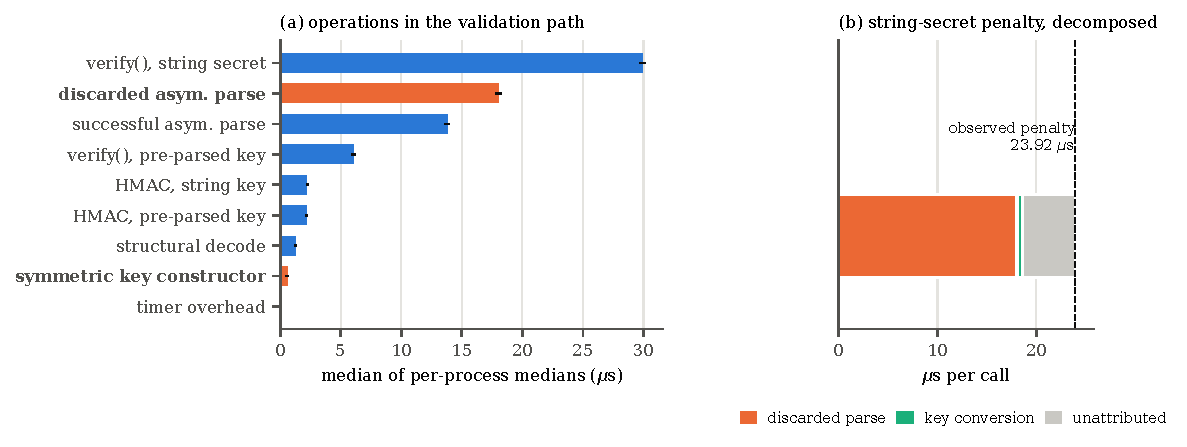
\includegraphics[width=\textwidth]{fig_decomposition.pdf}
\DIFdelbeginFL %DIFDELCMD < \caption{(a) Every operation in Table~\ref{tab:host}, on a linear scale, with
%DIFDELCMD < the two components the paper turns on emphasised; whiskers are the 95\%
%DIFDELCMD < percentile bootstrap intervals over \HostInvocations{} processes. (b) The
%DIFDELCMD < \HostStringPenalty~$\mu$s penalty for supplying a string secret rather than a
%DIFDELCMD < pre-parsed key, decomposed. The three segments are medians of per-round paired
%DIFDELCMD < differences, not a partition of a single measurement, and they do not sum to the
%DIFDELCMD < penalty: the \DecompResidual~$\mu$s remainder is unattributed
%DIFDELCMD < (Section~\ref{sec:residual}). Both panels are generated from
%DIFDELCMD < \texttt{figures/data/} by \texttt{figures/make\_figures.py}~\cite{artifact2026}.}
%DIFDELCMD < %%%
\DIFdelendFL \DIFaddbeginFL \caption{(a) Every operation in Table~\ref{tab:host}, on a linear scale, with
the two components the paper turns on emphasised; whiskers are the 95\%
percentile bootstrap intervals over \HostInvocations{} processes. (b) The
\HostStringPenalty~$\mu$s penalty for supplying a string secret rather than a
pre-parsed key, decomposed. The three segments are medians of per-round paired
differences, not a partition of a single measurement, and they do not sum to the
penalty: the \DecompResidual~$\mu$s remainder is unattributed
(Section~\ref{sec:residual}).}
\DIFaddendFL \label{fig:decomposition}
\end{figure*}

The two emphasised rows are the result. The signature primitive costs
\HostHmacString~$\mu$s of a \HostJwtString~$\mu$s call. The conversion to which
the remainder had been attributed, including by us, costs
\HostCreateSecretKey~$\mu$s. The discarded attempt that precedes that conversion
costs \HostProbeThrows~$\mu$s, which is \HostProbeShareOfCall\% of the whole call
and its largest single component.

Supplying a pre-parsed key instead of a string reduces the call by
\HostStringPenalty~$\mu$s [\HostStringPenaltyCiLo, \HostStringPenaltyCiHi] over
\HostStringPenaltyRounds{} paired rounds.

\paragraph{The natural repair is also wrong.} Once the signature primitive is
shown to be small, one explanation for the remainder suggests itself immediately:
that the cost lies in converting key material from a string into a key object on
every call. It is the explanation we held before measuring it, and
Table~\ref{tab:host} refutes it. That conversion costs
\HostCreateSecretKey~$\mu$s, so the attribution is wrong by roughly the ratio
between that figure and \HostProbeThrows~$\mu$s.

A second observation is usually offered in support of the conversion account: an
asymmetry between HMAC and RSA costs, read as conversion being dearer than
parsing a PEM. It is backwards. A successful asymmetric parse costs
\HostProbeSucceeds~$\mu$s against \HostCreateSecretKey~$\mu$s for the
conversion. The real asymmetry is that the RSA path's parse \emph{succeeds},
making its cost useful work, while the HMAC path's fails, making it waste.

\DIFdelbegin %DIFDELCMD < \subsection{What the \texorpdfstring{\HostProbeThrows~$\mu$s}{18 us} does and
%DIFDELCMD < does not separate}%%%
\DIFdelend \DIFaddbegin \subsection{What the \texorpdfstring{\HostProbeThrows~$\mu$s}{18 us} is made
of}\DIFaddend \label{sec:granularity}

The \HostProbeThrows~$\mu$s is the cost of the discarded attempt taken whole. It
contains at least two things: the work OpenSSL performs before concluding that
the input is not an asymmetric key, and the construction and unwinding of the
exception that returns that conclusion to the library. \DIFdelbegin \DIFdel{We did not separate them.
We state this prominently because the distinction bears directly on the
mechanism, and because a reader could otherwise take the headline as an
attribution to exception machinery alone.
}%DIFDELCMD < 

%DIFDELCMD < %%%
\DIFdel{One bound is available from Table~\ref{tab:host} and we state it as a bound
rather than as a
decomposition. A }\DIFdelend \DIFaddbegin \DIFadd{An earlier version of
this paper could only bound the split, from the observation that a
}\DIFaddend \emph{successful} asymmetric parse --- the same entry point, reaching a
conclusion \DIFdelbegin \DIFdel{, }\DIFdelend and throwing nothing --- costs \HostProbeSucceeds~$\mu$s\DIFdelbegin \DIFdel{. The failing parse costs }%DIFDELCMD < \HostProbeThrows%%%
\DIFdel{~$\mu$s. The
two paths are not identical in the work they perform before diverging, so the }%DIFDELCMD < \ProbeThrowsMinusSucceeds%%%
\DIFdelend \DIFaddbegin \DIFadd{, the same
order as the failing one. Table~\ref{tab:decomp} replaces the bound with a
decomposition, combining the C measurement of the same OpenSSL release
(Section~\ref{sec:c-method}) with the exception baseline
(Section~\ref{sec:exc-method}) on six official runtimes.
}

\begin{table*}[!t]
\caption{The discarded attempt decomposed, per runtime, in $\mu$s (x86\_64).
\emph{Probe}: \texttt{createPublicKey(secret)} inside Node, thrown and caught.
\emph{C parse}: the same OpenSSL calls issued from C against the OpenSSL
release that runtime bundles, built from source. \emph{V8 exception}: an
\texttt{Error} of the same shape, message and properties thrown from
\ExcDepth{} frames and discarded, with no OpenSSL call. \emph{Binding}: the
probe less the other two; its interval, from independent resampling of the
three runs, is in the replication package. Medians of per-process medians
over \ExcInvocations{} processes (probe, exception) and \CProbeInvocations{}
processes (C). The C column uses a stock build of each release, not Node's own
build of it, so the binding column is approximate (Section~\ref{sec:threats}).}
\label{tab:decomp}
\begin{tabular}{@{}llrrrr@{}}
\toprule
Runtime & OpenSSL & Probe & C parse & V8 exception & Binding \\
\midrule
Node \RtEighteenLiteral & \RtEighteenOpenssl & \RtEighteenProbe & \RtEighteenDecompC & \RtEighteenExcNodeLike & \RtEighteenDecompLeftover \\
Node \RtTwentyLiteral & \RtTwentyOpenssl & \RtTwentyProbe & \RtTwentyDecompC & \RtTwentyExcNodeLike & \RtTwentyDecompLeftover \\
Node \RtTwentyThreeLiteral & \RtTwentyThreeOpenssl & \RtTwentyThreeProbe & \RtTwentyThreeDecompC & \RtTwentyThreeExcNodeLike & \RtTwentyThreeDecompLeftover \\
Node \RtTwentyTwoLiteral & \RtTwentyTwoOpenssl & \RtTwentyTwoProbe & \RtTwentyTwoDecompC & \RtTwentyTwoExcNodeLike & \RtTwentyTwoDecompLeftover \\
Node \RtTwentyFourLiteral & \RtTwentyFourOpenssl & \RtTwentyFourProbe & \RtTwentyFourDecompC & \RtTwentyFourExcNodeLike & \RtTwentyFourDecompLeftover \\
Node \RtTwentySixLiteral & \RtTwentySixOpenssl & \RtTwentySixProbe & \RtTwentySixDecompC & \RtTwentySixExcNodeLike & \RtTwentySixDecompLeftover \\
\bottomrule
\end{tabular}
\end{table*}

\DIFadd{Three things follow. First, on every runtime bundling OpenSSL~3.0 the C parse
alone matches the probe to within a few percent --- }\RtEighteenDecompCPct\DIFadd{\% of
it under Node }\RtEighteenLiteral{} \DIFadd{and }\RtTwentyThreeDecompCPct\DIFadd{\% under Node
}\RtTwentyThreeLiteral\DIFadd{, the excess over 100\% being the difference between our
build of the release and Node's. There the discarded attempt }\emph{\DIFadd{is}} \DIFadd{the
OpenSSL parse, and it would cost the same with no JavaScript engine present.
Second, the exception is small and nearly constant across runtimes: the
Node-shaped error costs }\RtEighteenExcNodeLike\DIFaddend ~$\mu$s \DIFdelbegin \DIFdel{difference cannot be read directly as the price
of the exception. What it
does show is that a quantity of }\DIFdelend \DIFaddbegin \DIFadd{under Node
}\RtEighteenLiteral{} \DIFadd{and }\RtTwentySixExcNodeLike\DIFadd{~$\mu$s under Node
}\RtTwentySixLiteral{} \DIFadd{(}\RtEighteenDecompExcPct\DIFadd{\% and
}\RtTwentySixDecompExcPct\DIFadd{\% of the respective probes), and roughly half of it
is stack capture (with capture disabled, }\RtEighteenExcNoStack{} \DIFadd{and
}\RtTwentySixExcNoStack\DIFadd{~$\mu$s). Disabling stack capture for the real probe
saves }\RtEighteenStackCapture\DIFadd{~$\mu$s and }\RtTwentySixStackCapture\DIFadd{~$\mu$s on
the same two runtimes, }\DIFaddend the same order as \DIFdelbegin \DIFdel{a
complete successful parse is spent on the failing path before any exception
exists, which is why we describe the component as }\DIFdelend \DIFaddbegin \DIFadd{the synthetic figure. Third, on
runtimes bundling OpenSSL~3.5, where the parse is cheap, the three parts are of
comparable size: under Node }\RtTwentySixLiteral{} \DIFadd{the parse is
}\RtTwentySixDecompCPct\DIFadd{\% of the probe, the exception }\RtTwentySixDecompExcPct\DIFadd{\%
and the binding }\RtTwentySixDecompLeftoverPct\DIFadd{\%.
}

\DIFadd{This is why the component is named }\DIFaddend a discarded \emph{parse attempt} rather than
\DIFdelbegin \DIFdel{as }\DIFdelend a discarded exception. \DIFdelbegin %DIFDELCMD < 

%DIFDELCMD < %%%
\DIFdel{Section~\ref{sec:gaps} records that we found no V8-specific baseline for
}\texttt{\DIFdel{Error}} %DIFAUXCMD
\DIFdel{construction cost against which to calibrate the remainder.
Separating the two components requires either an instrument inside OpenSSL or a
condition that reaches the same failure without constructing a JavaScript
exception ; we have neither, and we make no claim at that granularity}\DIFdelend \DIFaddbegin \DIFadd{Where it is expensive the exception is about a
hundredth of it, and even where it is cheap the exception is a fifth. These
runtimes are Linux builds on x86\_64; the ARM64 host figure of
Table~\ref{tab:host} was not itself decomposed this way, and its
}\HostProbeThrows\DIFadd{~$\mu$s is of the same order as the OpenSSL~3.5 rows here, not
the OpenSSL~3.0 rows}\DIFaddend .

\subsection{The parts do not account for all of it}\label{sec:residual}

If the penalty for supplying a string were exactly the discarded attempt plus the
conversion, the two would sum to it. They do not, quite:

\begin{center}
\begin{tabular}{@{}lr@{}}
\toprule
observed penalty              & \DecompObserved~$\mu$s \\
discarded parse $+$ conversion & \DecompPredicted~$\mu$s \\
residual                      & \DecompResidual~$\mu$s \\
\bottomrule
\end{tabular}
\end{center}

All three quantities are medians of per-round paired differences, per
Section~\ref{sec:unit}. The residual's interval,
[\DecompResidualCiLo, \DecompResidualCiHi], excludes zero. The two measured
parts therefore account for \DecompExplainedPct\% and not more; the remainder
lies in the library's own type and claim checking along the non-pre-parsed path.
We report it rather than absorbing it into the headline, because a decomposition
whose parts are declared to sum exactly to the whole has usually not been
checked.

The pre-parsed path carries a smaller unexplained remainder of the same kind, and
we record it for consistency rather than leaving the asymmetry unremarked:
\texttt{verify()} with a pre-parsed key costs \HostJwtPreparsed~$\mu$s against
\HostDecodeOnly~$\mu$s of structural decode plus \HostHmacKeyObject~$\mu$s of
HMAC, leaving roughly \PreparsedUnattributed~$\mu$s unattributed. Neither
residual was measured directly; both are the subject of conditions we did not
run, and both are stated as unattributed rather than assigned.

\subsection{Confirmation without differencing}

The decomposition reaches its conclusion by subtracting conditions --- the same
inference style this paper criticises elsewhere. It is therefore checked against
V8's sampling profiler, which attributes self time to named frames with no
arithmetic on our part. At \ProfIterations{} iterations per run and
\ProfRepeats{} runs per environment, matched so the percentages are comparable,
the asymmetric key parse accounts for a median \ProfHostPct\% of self time on
the host (range \ProfHostPctLo--\ProfHostPctHi{} across runs),
\ProfEighteenPct\% (\ProfEighteenPctLo--\ProfEighteenPctHi) under Node
\NodeEighteenNodeMajor, and \ProfTwentySixPct\%
(\ProfTwentySixPctLo--\ProfTwentySixPctHi) under Node
\NodeTwentySixMuslNodeMajor. The frame does not appear among the top frames of
the pre-parsed path in any environment.

Two methods, one answer. We rely on the ordering and the dominance rather than on
the exact percentages: sampling attribution depends on rate and on what else the
process is doing.

%% ============================================================================
\DIFdelbegin %DIFDELCMD < \section{RQ2: What the magnitude co-varies with}%%%
\DIFdelend \DIFaddbegin \section{RQ2: What governs the magnitude}\DIFaddend \label{sec:rq2}

Table~\ref{tab:matrix} varies the runtime with containerisation held constant,
and Figure~\ref{fig:matrix} plots the two columns that matter.

\DIFdelbegin %DIFDELCMD < \begin{table}[t]
%DIFDELCMD < \caption{The same measurement across four container runtimes on one machine,
%DIFDELCMD < \MatrixInvocations{} processes each of \MatrixCallsPerInvocation{} calls. The
%DIFDELCMD < host row is from Table~\ref{tab:host} and is not containerised; its OpenSSL
%DIFDELCMD < version is marked n/r because that run predates the per-measurement OpenSSL field
%DIFDELCMD < and the host's OpenSSL has since changed, so no version can be recorded for it
%DIFDELCMD < after the fact (Section~\ref{sec:threats}).}
%DIFDELCMD < \label{tab:matrix}
%DIFDELCMD < \footnotesize\setlength{\tabcolsep}{3.5pt}
%DIFDELCMD < \begin{tabular}{@{}lllrr@{}}
%DIFDELCMD < \toprule
%DIFDELCMD < Runtime & OpenSSL & V8 & Disc.\ parse & Pre-parsed \\
%DIFDELCMD <         &         &    & ($\mu$s)     & \texttt{verify()} \\
%DIFDELCMD < \midrule
%DIFDELCMD < Node \NodeEighteenNodeMajor, musl        & \NodeEighteenOpensslLiteral     & \NodeEighteenVeight     & \NodeEighteenProbeThrows     & \NodeEighteenJwtPreparsed \\
%DIFDELCMD < Node \NodeTwentyNodeMajor, musl          & \NodeTwentyOpensslLiteral       & \NodeTwentyVeight       & \NodeTwentyProbeThrows       & \NodeTwentyJwtPreparsed \\
%DIFDELCMD < Node \NodeTwentySixMuslNodeMajor, musl   & \NodeTwentySixMuslOpensslLiteral & \NodeTwentySixMuslVeight & \NodeTwentySixMuslProbeThrows & \NodeTwentySixMuslJwtPreparsed \\
%DIFDELCMD < Node \NodeTwentySixGlibcNodeMajor, glibc & \NodeTwentySixGlibcOpensslLiteral & \NodeTwentySixGlibcVeight & \NodeTwentySixGlibcProbeThrows & \NodeTwentySixGlibcJwtPreparsed \\
%DIFDELCMD < host (no container)                      & n/r                             & \HostVeight             & \HostProbeThrows             & \HostJwtPreparsed \\
%DIFDELCMD < \bottomrule
%DIFDELCMD < \end{tabular}
%DIFDELCMD < \end{table}
%DIFDELCMD < %%%
\DIFdelend \DIFaddbegin \begin{table}[!htbp]
\caption{The same measurement across four container runtimes on one machine,
\MatrixInvocations{} processes each of \MatrixCallsPerInvocation{} calls. The
\emph{Disc.\ parse}: the discarded asymmetric parse; \emph{Pre-parsed}:
\texttt{verify()} with a pre-parsed key. $^{\ddagger}$The host row is from
Table~\ref{tab:host} and is not containerised.
$^{\dagger}$Inferred from the run timestamp, not recorded per row: that run
predates the per-measurement OpenSSL field (Section~\ref{sec:threats}).}
\label{tab:matrix}
\footnotesize\setlength{\tabcolsep}{1.6pt}
\begin{tabular}{@{}lllrr@{}}
\toprule
Runtime & OpenSSL & V8 & Disc.\ parse & Pre-parsed \\
        &         &    & ($\mu$s)     & ($\mu$s) \\
\midrule
Node \NodeEighteenNodeMajor{} musl        & \NodeEighteenOpensslLiteral       & \NodeEighteenVeight       & \NodeEighteenProbeThrows       & \NodeEighteenJwtPreparsed \\
Node \NodeTwentyNodeMajor{} musl          & \NodeTwentyOpensslLiteral         & \NodeTwentyVeight         & \NodeTwentyProbeThrows         & \NodeTwentyJwtPreparsed \\
Node \NodeTwentySixMuslNodeMajor{} musl   & \NodeTwentySixMuslOpensslLiteral  & \NodeTwentySixMuslVeight  & \NodeTwentySixMuslProbeThrows  & \NodeTwentySixMuslJwtPreparsed \\
Node \NodeTwentySixGlibcNodeMajor{} glibc & \NodeTwentySixGlibcOpensslLiteral & \NodeTwentySixGlibcVeight & \NodeTwentySixGlibcProbeThrows & \NodeTwentySixGlibcJwtPreparsed \\
host$^{\ddagger}$                         & \HostOpensslInferred$^{\dagger}$  & \HostVeight               & \HostProbeThrows               & \HostJwtPreparsed \\
\bottomrule
\end{tabular}
\end{table}
\DIFaddend 

\DIFdelbegin %DIFDELCMD < \begin{figure*}[t]
%DIFDELCMD < %%%
\DIFdelendFL \DIFaddbeginFL \begin{figure*}[!t]
\DIFaddendFL \centering
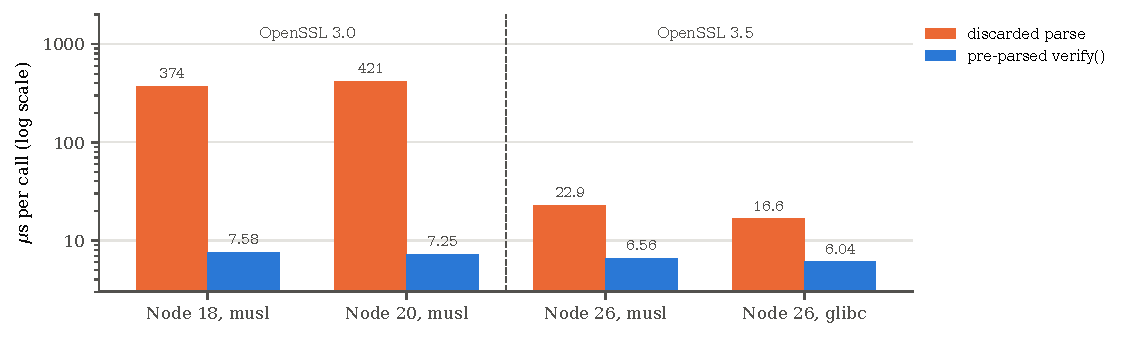
\includegraphics[width=\textwidth]{fig_runtime_matrix.pdf}
\DIFdelbeginFL %DIFDELCMD < \caption{The four container rows of Table~\ref{tab:matrix} on a logarithmic
%DIFDELCMD < axis. The discarded parse spans \SpanProbeThrows$\times$ across images while the
%DIFDELCMD < pre-parsed call spans \SpanJwtPreparsed$\times$. The dashed rule marks the
%DIFDELCMD < OpenSSL series boundary; it is \emph{not} a controlled boundary, because the two
%DIFDELCMD < fast images also carry a newer engine and a different build
%DIFDELCMD < (Section~\ref{sec:cannot-separate}). The uncontainerised host row is omitted
%DIFDELCMD < because its comparison with the container rows is confounded. Generated by
%DIFDELCMD < \texttt{figures/make\_figures.py}~\cite{artifact2026}.}
%DIFDELCMD < %%%
\DIFdelendFL \DIFaddbeginFL \caption{The four container rows of Table~\ref{tab:matrix} on a logarithmic
axis. The discarded parse spans \SpanProbeThrows$\times$ across images while the
pre-parsed call spans \SpanJwtPreparsed$\times$. The dashed rule marks the
OpenSSL series boundary. Within this matrix it is not a controlled boundary,
because the two fast images also carry a newer engine and a different build
(Section~\ref{sec:cannot-separate}); Section~\ref{sec:rq2-causal} controls it. The uncontainerised host row is omitted
because its comparison with the container rows is confounded.}
\DIFaddendFL \label{fig:matrix}
\end{figure*}

\subsection{Engine major version does not distinguish the two slow runtimes}

Node \NodeEighteenNodeMajor{} and Node \NodeTwentyNodeMajor{} ship V8
\NodeEighteenVeight{} and \NodeTwentyVeight{} --- different major versions of the
engine --- and share the OpenSSL \NodeEighteenOpensslSeries{} series. Both pay of
order \NodeEighteenProbeThrows--\NodeTwentyProbeThrows~$\mu$s. Node
\NodeTwentySixMuslNodeMajor{} ships OpenSSL \NodeTwentySixMuslOpensslSeries{} and
pays \NodeTwentySixMuslProbeThrows~$\mu$s on the same libc. Within the OpenSSL
\NodeEighteenOpensslSeries{} series, then, changing the engine's major version
does not move the quantity; had Node \NodeTwentyNodeMajor{} been fast, the
attribution would have been to the engine.

\subsection{What this design cannot separate}\label{sec:cannot-separate}

That argument establishes a negative within one OpenSSL series. It does not
establish the positive attribution for the change between series, and we state
the limitation rather than leaving it implicit.

The fast rows are Node \NodeTwentySixMuslNodeMajor. They carry OpenSSL
\NodeTwentySixMuslOpensslSeries{} \emph{and} V8 \NodeTwentySixMuslVeight{}
\emph{and} every other change in that build. OpenSSL version is therefore
perfectly confounded with engine version and with build configuration across the
\NodeEighteenOpensslSeries--\NodeTwentySixMuslOpensslSeries{} boundary. Nothing
in this matrix can separate them. The absence of variation between V8
\NodeEighteenVeight{} and V8 \NodeTwentyVeight{} does not license the inference
that V8 \NodeTwentySixMuslVeight{} is also irrelevant; that is a different
comparison, and we did not make it.

What the matrix supports \DIFaddbegin \DIFadd{on its own }\DIFaddend is the following, and no more: the
magnitude co-varies with the bundled OpenSSL version across four images; the two
slow images differ in engine major version and do not differ in magnitude; and
the two libc variants of one image differ by less than the difference between
series. Separating OpenSSL from the engine requires a crossed design --- a
\DIFdelbegin \DIFdel{single Node version
linked against both OpenSSLseries}\DIFdelend \DIFaddbegin \DIFadd{runtime pairing a newer engine with an older OpenSSL}\DIFaddend , or the parse measured
outside Node entirely\DIFdelbegin \DIFdel{--- which we did not run. We therefore write }\DIFdelend \DIFaddbegin \DIFadd{. An earlier version of this paper had neither and wrote
}\DIFaddend \emph{co-varies with} throughout\DIFdelbegin \DIFdel{,
including in the abstract and the conclusion, and we draw no causal conclusion
about OpenSSL from this data. }%DIFDELCMD < 

%DIFDELCMD < %%%
\DIFdel{The engineering evidence cited in Section~\ref{sec:gaps} proposes a mechanism for
such a regression. We do not adopt it,
for the reason given there: it is not
peer-reviewed and was not produced under a protocol we can assess}\DIFdelend \DIFaddbegin \DIFadd{. Section~\ref{sec:rq2-causal} reports both,
and it is on them, not on this matrix, that the causal wording now used rests}\DIFaddend .

\subsection{The effect is confined to key parsing}

Across the four container rows, pre-parsed validation spans
\SpanJwtPreparsed$\times$, the HMAC primitive \SpanHmacString$\times$ and
structural decode \SpanDecodeOnly$\times$. The discarded parse spans
\SpanProbeThrows$\times$. The successful parse moves with it
(\SpanProbeSucceeds$\times$), so this is the cost of key parsing in general
rather than anything peculiar to the failure path. The failure is simply the case
in which an application pays that cost on every request for a result it discards.

\subsection{What this design does not isolate}

A reader may notice that the uncontainerised host row is of the same order as the
Node \NodeTwentySixGlibcNodeMajor{} container row. That comparison is confounded
and we draw no conclusion about containerisation from it: the host runs a
different operating system from the containers, so operating system, C library
and Node build all change alongside the container boundary. Isolating
containerisation would require a Linux-native baseline, which we did not obtain.
The claims above concern only the four container rows, among which
containerisation is constant.

\DIFaddbegin \subsection{Caused by OpenSSL: the parse without an engine}\label{sec:rq2-causal}

\DIFadd{Table~\ref{tab:cprobe} removes Node entirely: the OpenSSL calls
}\texttt{\DIFadd{createPublicKey()}} \DIFadd{makes for an HMAC secret, issued from C against
}\CProbeVersionCount{} \DIFadd{OpenSSL releases built identically.
}

\begin{table*}[!t]
\caption{The failed asymmetric parse issued from C, with no JavaScript engine,
against \CProbeVersionCount{} OpenSSL releases built from source with one
compiler and one set of flags (x86\_64), in $\mu$s. Medians of per-process
medians over \CProbeInvocations{} processes of \CProbeCallsPerInvocation{}
calls. \emph{Full}: everything \texttt{createPublicKey()} asks of OpenSSL for
an HMAC secret, including the error-string drain; 95\% intervals for it are in
the replication package and are within \CFullCiMaxHalfWidthPct\% of the median for every release.
Its parts follow. \emph{Successful parse}: an RSA-2048 public key through the
same path, for comparison.}
\label{tab:cprobe}
\begin{tabular}{@{}lrrrrr@{}}
\toprule
        &      & Private-key & Public-key & Error   & Successful \\
OpenSSL & Full & parse       & scans      & strings & parse \\
\midrule
\CVersionLiteralVThreeZeroSixteen & \CFullVThreeZeroSixteen & \CPrivateParseVThreeZeroSixteen & \CPublicTriesVThreeZeroSixteen & \CErrorStringsVThreeZeroSixteen & \CSpkiOkVThreeZeroSixteen \\
\CVersionLiteralVThreeZeroNineteen & \CFullVThreeZeroNineteen & \CPrivateParseVThreeZeroNineteen & \CPublicTriesVThreeZeroNineteen & \CErrorStringsVThreeZeroNineteen & \CSpkiOkVThreeZeroNineteen \\
\CVersionLiteralVThreeOneEight & \CFullVThreeOneEight & \CPrivateParseVThreeOneEight & \CPublicTriesVThreeOneEight & \CErrorStringsVThreeOneEight & \CSpkiOkVThreeOneEight \\
\CVersionLiteralVThreeTwoSix & \CFullVThreeTwoSix & \CPrivateParseVThreeTwoSix & \CPublicTriesVThreeTwoSix & \CErrorStringsVThreeTwoSix & \CSpkiOkVThreeTwoSix \\
\CVersionLiteralVThreeThreeFive & \CFullVThreeThreeFive & \CPrivateParseVThreeThreeFive & \CPublicTriesVThreeThreeFive & \CErrorStringsVThreeThreeFive & \CSpkiOkVThreeThreeFive \\
\CVersionLiteralVThreeFourThree & \CFullVThreeFourThree & \CPrivateParseVThreeFourThree & \CPublicTriesVThreeFourThree & \CErrorStringsVThreeFourThree & \CSpkiOkVThreeFourThree \\
\CVersionLiteralVThreeFiveEight & \CFullVThreeFiveEight & \CPrivateParseVThreeFiveEight & \CPublicTriesVThreeFiveEight & \CErrorStringsVThreeFiveEight & \CSpkiOkVThreeFiveEight \\
\CVersionLiteralVThreeSixOne & \CFullVThreeSixOne & \CPrivateParseVThreeSixOne & \CPublicTriesVThreeSixOne & \CErrorStringsVThreeSixOne & \CSpkiOkVThreeSixOne \\
\bottomrule
\end{tabular}
\end{table*}

\DIFadd{In plain C the failure costs }\CFullVThreeZeroSixteen\DIFadd{~$\mu$s on OpenSSL }\CVersionLiteralVThreeZeroSixteen{}
\DIFadd{and }\CFullVThreeFiveEight\DIFadd{~$\mu$s on }\CVersionLiteralVThreeFiveEight\DIFadd{, a ratio of }\CFullRatioOldNew{}
[\CFullRatioOldNewCiLo\DIFadd{, }\CFullRatioOldNewCiHi]\DIFadd{. Nothing else differs between
those two measurements: the program, the compiler, the flags, the machine and
the protocol are the same. The magnitude is therefore }\emph{\DIFadd{caused}} \DIFadd{by the
OpenSSL release. That is a claim about this code path in these releases; it
says nothing about OpenSSL performance generally.
}

\DIFadd{The table also says where in OpenSSL the cost lives and when it went away.
Almost all of it is the private-key parse --- }\CPrivateShareVThreeZeroSixteen\DIFadd{\%
of the full sequence on }\CVersionLiteralVThreeZeroSixteen{} \DIFadd{--- the step at which OpenSSL~3 hands the input
to its provider-based decoders; the three public-key scans reject the input at
the PEM header and are cheap in every release, and the error strings cost under
a microsecond. The fall came in two steps: to }\CFullVThreeOneEight\DIFadd{~$\mu$s in
}\CVersionLiteralVThreeOneEight\DIFadd{, and to }\CFullVThreeTwoSix\DIFadd{~$\mu$s in }\CVersionLiteralVThreeTwoSix\DIFadd{, after which it is flat to
within a few microseconds through }\CProbeVersionLast\DIFadd{. We measured the steps,
not the source changes that produced them; identifying those would take a
bisection of the OpenSSL history that we have not done. A successful parse of
real key material fell with it, which is why the effect is confined to key
parsing in general rather than to the failure path.
}

\paragraph{Engine and library crossed.} \DIFadd{The official runtimes of
Section~\ref{sec:exc-method} contain the pairing stock container images lack:
Node }\RtTwentyTwoLiteral{} \DIFadd{ships V8 }\RtTwentyTwoVeightFull{} \DIFadd{with OpenSSL
}\RtTwentyTwoOpenssl\DIFadd{, while Node }\RtTwentyThreeLiteral{} \DIFadd{ships the }\emph{\DIFadd{newer}}
\DIFadd{V8 }\RtTwentyThreeVeightFull{} \DIFadd{with the }\emph{\DIFadd{older}} \DIFadd{OpenSSL
}\RtTwentyThreeOpenssl\DIFadd{. The probe costs }\RtTwentyTwoProbe\DIFadd{~$\mu$s on the first
and }\RtTwentyThreeProbe\DIFadd{~$\mu$s on the second. The Node }\NodeEighteenNodeMajor\DIFadd{/}\NodeTwentyNodeMajor{} \DIFadd{pair of
Table~\ref{tab:matrix} showed that a change of engine at a fixed OpenSSL series
leaves the cost where it was; this pair shows that a newer engine does not
rescue an older OpenSSL. Together with the C measurement, the engine is
excluded from both directions.
}

\subsection{A second architecture}\label{sec:rq2-arch}

\DIFadd{Table~\ref{tab:arch} repeats the runtime matrix, with the same images and
scripts, on x86\_64 (Section~\ref{sec:arch-method}). Absolute values are not
compared across the two machines; the question is whether the ordering holds.
}

\begin{table*}[!t]
\caption{The runtime matrix of Table~\ref{tab:matrix} on two architectures,
same images and scripts, in $\mu$s. ARM64: \MatrixInvocations{} processes of
\MatrixCallsPerInvocation{} calls. x86\_64, a shared cloud virtual machine:
\XmInvocations{} processes of \XmCallsPerInvocation{} calls. Absolute values
are not comparable across the two machines.}
\label{tab:arch}
\begin{tabular}{@{}llrrrr@{}}
\toprule
 & & \multicolumn{2}{c}{Discarded parse} & \multicolumn{2}{c}{Pre-parsed \texttt{verify()}} \\
Image & OpenSSL & ARM64 & x86\_64 & ARM64 & x86\_64 \\
\midrule
\texttt{node:18.20.8-alpine} & \NodeEighteenOpensslLiteral & \NodeEighteenProbeThrows & \XmEighteenProbeThrows & \NodeEighteenJwtPreparsed & \XmEighteenJwtPreparsed \\
\texttt{node:20-alpine} & \NodeTwentyOpensslLiteral & \NodeTwentyProbeThrows & \XmTwentyProbeThrows & \NodeTwentyJwtPreparsed & \XmTwentyJwtPreparsed \\
\texttt{node:26.6.0-alpine} & \NodeTwentySixMuslOpensslLiteral & \NodeTwentySixMuslProbeThrows & \XmTwentySixMuslProbeThrows & \NodeTwentySixMuslJwtPreparsed & \XmTwentySixMuslJwtPreparsed \\
\texttt{node:26.6.0-bookworm} & \NodeTwentySixGlibcOpensslLiteral & \NodeTwentySixGlibcProbeThrows & \XmTwentySixGlibcProbeThrows & \NodeTwentySixGlibcJwtPreparsed & \XmTwentySixGlibcJwtPreparsed \\
\bottomrule
\end{tabular}
\end{table*}

\DIFadd{The property the attribution rests on --- every OpenSSL~3.0 image slower than
every OpenSSL~3.5 image --- }\XmSeriesSplitHolds{} \DIFadd{on both architectures. The
strict rank order does not: the two OpenSSL~3.0 images, Node
}\NodeEighteenNodeMajor{} \DIFadd{and Node }\NodeTwentyNodeMajor\DIFadd{, exchange places between
ARM64 and x86\_64. Their difference is small against the gap between series on
either machine, and no claim in this paper depends on their relative order. On x86\_64 the discarded parse spans
}\XmSpanProbeThrows\DIFadd{$\times$ across the images while pre-parsed validation spans
}\XmSpanJwtPreparsed\DIFadd{$\times$, against }\SpanProbeThrows\DIFadd{$\times$ and
}\SpanJwtPreparsed\DIFadd{$\times$ on ARM64. The host decomposition of
Table~\ref{tab:host} was repeated too (Node }\XhNode\DIFadd{, OpenSSL }\XhOpenssl\DIFadd{): the
discarded parse is }\XhProbeThrows\DIFadd{~$\mu$s of a }\XhJwtString\DIFadd{~$\mu$s call
(}\XhProbeShareOfCall\DIFadd{\%), the symmetric constructor }\XhCreateSecretKey\DIFadd{~$\mu$s
and the HMAC primitive }\XhHmacString\DIFadd{~$\mu$s, so the component ordering of
Table~\ref{tab:host} holds there as well. The full x86\_64 host table is in the
replication package.
}

\DIFaddend %% ============================================================================
\section{RQ3: Deployment and prevalence}\label{sec:rq3}

\subsection{In-situ cost across arrival rates}\label{sec:insitu}

The deployed service was driven at seven arrival rates, each measured by the
paired-scrape difference of Section~\ref{sec:insitu-method}, with the whole sweep
run ascending and then descending on one process. Table~\ref{tab:insitu} reports
the range across the two passes at each rate for the configuration the service
deploys, a string secret, and Figure~\ref{fig:insitu} plots it.

\DIFdelbegin %DIFDELCMD < \begin{table}[t]
%DIFDELCMD < \caption{In-situ validation cost with a string secret, by arrival rate. The two
%DIFDELCMD < columns are the ascending and the descending pass over the same seven rates on
%DIFDELCMD < one process; each is a single window, and the pair is two observations rather
%DIFDELCMD < than an interval. Host load average during each window is committed with the
%DIFDELCMD < measurement.}
%DIFDELCMD < \label{tab:insitu}
%DIFDELCMD < \begin{tabular}{@{}lrr@{}}
%DIFDELCMD < \toprule
%DIFDELCMD < Arrival rate & \multicolumn{2}{c}{Mean per call ($\mu$s)} \\
%DIFDELCMD < (requests/s) & ascending & descending \\
%DIFDELCMD < \midrule
%DIFDELCMD < \InsituRateA & \InsituStringAscA & \InsituStringDescA \\
%DIFDELCMD < \InsituRateB & \InsituStringAscB & \InsituStringDescB \\
%DIFDELCMD < \InsituRateC & \InsituStringAscC & \InsituStringDescC \\
%DIFDELCMD < \InsituRateD & \InsituStringAscD & \InsituStringDescD \\
%DIFDELCMD < \InsituRateE & \InsituStringAscE & \InsituStringDescE \\
%DIFDELCMD < \InsituRateF & \InsituStringAscF & \InsituStringDescF \\
%DIFDELCMD < \InsituRateG & \InsituStringAscG & \InsituStringDescG \\
%DIFDELCMD < \bottomrule
%DIFDELCMD < \end{tabular}
%DIFDELCMD < \end{table}
%DIFDELCMD < %%%
\DIFdelend \DIFaddbegin \begin{table}[!htbp]
\caption{In-situ validation cost with a string secret, by arrival rate. The two
columns are the ascending and the descending pass over the same seven rates on
one process; each is a single window, and the pair is two observations rather
than an interval. Host load average during each window is committed with the
measurement.}
\label{tab:insitu}
\begin{tabular}{@{}lrr@{}}
\toprule
Arrival rate & \multicolumn{2}{c}{Mean per call ($\mu$s)} \\
(requests/s) & ascending & descending \\
\midrule
\InsituRateA & \InsituStringAscA & \InsituStringDescA \\
\InsituRateB & \InsituStringAscB & \InsituStringDescB \\
\InsituRateC & \InsituStringAscC & \InsituStringDescC \\
\InsituRateD & \InsituStringAscD & \InsituStringDescD \\
\InsituRateE & \InsituStringAscE & \InsituStringDescE \\
\InsituRateF & \InsituStringAscF & \InsituStringDescF \\
\InsituRateG & \InsituStringAscG & \InsituStringDescG \\
\bottomrule
\end{tabular}
\end{table}
\DIFaddend 

\DIFdelbegin %DIFDELCMD < \begin{figure}[t]
%DIFDELCMD < %%%
\DIFdelendFL \DIFaddbeginFL \begin{figure}[!htbp]
\DIFaddendFL \centering
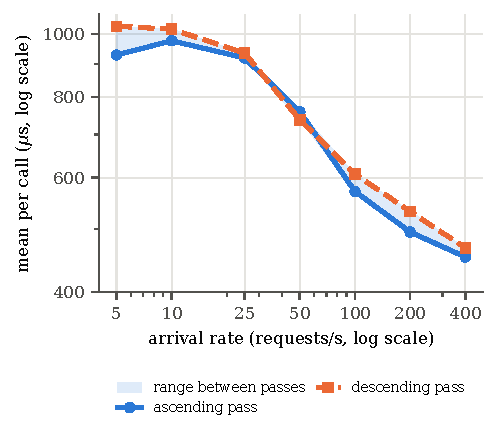
\includegraphics[width=\columnwidth]{fig_insitu_rate.pdf}
\DIFdelbeginFL %DIFDELCMD < \caption{In-situ validation cost against arrival rate, string secret. The two
%DIFDELCMD < passes are drawn separately rather than averaged: Section~\ref{sec:drift} reports
%DIFDELCMD < that they differ systematically, and averaging would conceal that. The shaded
%DIFDELCMD < band is the range between the passes, which is two observations rather than an
%DIFDELCMD < interval. Generated by
%DIFDELCMD < \texttt{figures/make\_figures.py}~\cite{artifact2026}.}
%DIFDELCMD < %%%
\DIFdelendFL \DIFaddbeginFL \caption{In-situ validation cost against arrival rate, string secret. The two
passes are drawn separately rather than averaged: Section~\ref{sec:drift} reports
that they differ systematically, and averaging would conceal that. The shaded
band is the range between the passes, which is two observations rather than an
interval.}
\DIFaddendFL \label{fig:insitu}
\end{figure}

One observation follows, and it is the one this section claims: the cost is
present in deployment and is far larger than the isolated host figure of
Table~\ref{tab:host}, consistent with Section~\ref{sec:rq2} in that the deployed
runtime is the one carrying the older OpenSSL.

Two things visible in Table~\ref{tab:insitu} \DIFdelbegin \DIFdel{are }\emph{\DIFdel{not}} %DIFAUXCMD
\DIFdel{claimed}\DIFdelend \DIFaddbegin \DIFadd{need care}\DIFaddend , and we set them out
explicitly.

\DIFdelbegin %DIFDELCMD < \paragraph{The magnitude is not reconciled with the microbenchmark.} %%%
\DIFdelend \DIFaddbegin \paragraph{Wall-clock exceeds the prediction; processor time does not.} \DIFaddend The
deployed runtime's discarded parse costs \NodeEighteenProbeThrows~$\mu$s
(Table~\ref{tab:matrix}), and the remainder of the validation path is of order
\NodeEighteenJwtPreparsed~$\mu$s, giving an expected total near
\InsituPredictedFromMatrix~$\mu$s. The \DIFdelbegin \DIFdel{observed figures }\DIFdelend \DIFaddbegin \DIFadd{wall-clock means observed across the
sweep }\DIFaddend are \InsituObservedLo--\InsituObservedHi~$\mu$s\DIFaddbegin \DIFadd{, exceeding that by
}\InsituUnaccountedLo\DIFadd{--}\InsituUnaccountedHi\DIFadd{~$\mu$s}\DIFaddend . Contention inflates a
duration rather than deflating it, so these are upper bounds\DIFdelbegin \DIFdel{and are notinconsistent
with the microbenchmark; but a gap of roughly
}%DIFDELCMD < \InsituUnaccountedLo%%%
\DIFdel{--}%DIFDELCMD < \InsituUnaccountedHi%%%
\DIFdel{~$\mu$s is unaccounted for, and we
report it as unaccounted rather than attributing it. It was not decomposed}\DIFdelend \DIFaddbegin \DIFadd{, and
Section~\ref{sec:abcorroboration} shows where the excess is not: measured as
processor time, the validation call costs within }\AbCpuVsPredictedPct\DIFadd{\% of the
prediction. The excess is therefore time the call spent off the processor on a
shared host, not additional work. We did not decompose that off-processor time
further, and no claim below depends on it}\DIFaddend .

\paragraph{The decline with arrival rate is not interpreted.} Cost falls
monotonically from \InsituStringAscA~$\mu$s at \InsituRateA~requests/s to
\InsituStringAscG~$\mu$s at \InsituRateG~requests/s. This is the opposite of what
contention alone would produce, and several mechanisms unrelated to validation
would produce it --- a fixed per-window overhead amortising over more calls,
processor frequency scaling and idle-state exit latency at low rates, cache and
branch-predictor residency, or continued tier-up in the engine. We did not run
the conditions that would distinguish them. We therefore report the numbers and
do not claim that validation cost depends on arrival rate; establishing that
would require varying window duration at fixed rate, pinning the frequency
governor, and extending warmup at low rates, none of which we did.

\subsection{The two passes differ systematically}\label{sec:drift}

Sweeping up and then down is not only replication; it detects warm-up, thermal
and hysteresis effects. If the difference between passes were noise, its sign
would alternate across rate points. It does not. In the string-secret sweep the
descending pass is slower at \InsituStringSameSign{} of \InsituStringPoints{}
rate points; in the pre-parsed sweep the descending pass is \emph{faster} at
\InsituPreparsedSameSign{} of \InsituPreparsedPoints. A consistent sign across
seven points is not what noise produces.

This has a direct consequence for how the ranges in Table~\ref{tab:insitu} should
be read. A systematic component means the two passes are not independent samples
of a common value, so the range between them understates uncertainty further than
a range of two already does. We therefore report ranges and draw no inference that
depends on their width. It is also a methodological finding in its own right: a
single-direction sweep would have produced a curve carrying a consistent bias with
no way to detect it.

\subsection{Host load, not the condition, drives the outliers}\label{sec:load}

Agreement between passes varies considerably across windows. We distinguish
\emph{relative} disagreement, the gap between passes as a fraction of their mean,
from \emph{absolute} disagreement, the gap in microseconds; the two behave
differently and the distinction carries this subsection.

The widest relative disagreement in the dataset and the tightest occur at the same
arrival rate in different sweeps. The wide one is the highest-load window in its
own sweep on the descending pass, though not on the ascending pass, whose maximum
load falls at a different rate. The tight one, at the same arrival rate in another
sweep, sits at a lower load on both passes and its two passes agree to within
\InsituTightestAgreement~$\mu$s. Relative disagreement therefore does not track
the condition under measurement.

We considered two alternative explanations for the relative asymmetry and reject
both. A small-mean effect would require absolute disagreement to be roughly
constant, so that its relative size grew only as means shrank; absolute
disagreement instead varies over three orders of magnitude and is largest where
the means are largest, which is the opposite pattern. A measurement floor would
require the affected values to sit at the instrument's resolution; they do not,
and in any case the means reported here are computed from the histogram's sum and
count rather than from its buckets, so bucket resolution cannot bound them.

The operative consequence is that in-situ figures are reported with the host load
recorded during their window, and comparisons between windows at different loads
are not treated as comparisons between conditions.

\DIFdelbegin %DIFDELCMD < \ifabdata
%DIFDELCMD < \subsection{Corroboration: the cost belongs to the validation
%DIFDELCMD < call}%%%
\DIFdelend \DIFaddbegin \subsection{Corroboration: the cost is processor time, and it matches the
prediction}\DIFaddend \label{sec:abcorroboration}
%DIF < % If an arm records PROCESS CPU TIME rather than wall clock, use this title
%DIF < % instead and swap in the commented paragraph below:
%DIF < % \subsection{Corroboration: the cost is real processor time}

An in-situ figure of this magnitude has two readings. Either it is work the
service performs, or it is \DIFdelbegin \DIFdel{an artefact of the surrounding measurement }\DIFdelend \DIFaddbegin \DIFadd{time the request spends waiting }\DIFaddend --- \DIFdelbegin \DIFdel{ambient handler cost that would be there without validation, or a property of
the instrumentrather than of the code}\DIFdelend \DIFaddbegin \DIFadd{queued behind
other requests, descheduled by a contended host, or inflated by the instrument}\DIFaddend .
We separate them with an A/B of the same service at one arrival rate, with
validation enabled in one window and disabled in the next\DIFdelbegin \DIFdel{under otherwise identical conditions}\DIFdelend \DIFaddbegin \DIFadd{, on the same pod
running the same image, and read the processor time the application container
was charged from its cgroup accounting rather than from a clock}\DIFaddend .
Table~\ref{tab:ab} reports it.

\DIFdelbegin %DIFDELCMD < \begin{table}[t]
%DIFDELCMD < \caption{Validation enabled against validation disabled, run
%DIFDELCMD < \texttt{\ABRunId}, at \ABRate~requests/s over \ABWindowSeconds~s per window.
%DIFDELCMD < The means time \ABQuantity, computed as the difference of the histogram's
%DIFDELCMD < \texttt{\_sum} divided by the difference of its \texttt{\_count}, as in
%DIFDELCMD < Section~\ref{sec:insitu-method}. \emph{Two caveats govern how this table may be
%DIFDELCMD < read.} First, the load figure is a single \texttt{uptime} sample taken at window
%DIFDELCMD < start --- the same quantity and capture path as the per-window load recorded
%DIFDELCMD < with the rate sweeps --- and not a mean over the window; no within-window load
%DIFDELCMD < series exists for these two runs. Second, the difference is a difference of two
%DIFDELCMD < window means, not the median of per-round paired differences used everywhere
%DIFDELCMD < else in this paper (Section~\ref{sec:unit}), because the two arms are separate
%DIFDELCMD < windows and cannot be paired. It is the only quantity in the paper of that kind,
%DIFDELCMD < and no other result depends on it.}
%DIFDELCMD < \label{tab:ab}
%DIFDELCMD < \small\setlength{\tabcolsep}{4pt}
%DIFDELCMD < \begin{tabular}{@{}lrrr@{}}
%DIFDELCMD < \toprule
%DIFDELCMD <             & Mean per call & Calls & Load at \\
%DIFDELCMD < Arm         & ($\mu$s)      &       & window start \\
%DIFDELCMD < \midrule
%DIFDELCMD < validation enabled  & \ABEnabledMean  & \ABEnabledCalls  & \ABEnabledLoad  \\
%DIFDELCMD < validation disabled & \ABDisabledMean & \ABDisabledCalls & \ABDisabledLoad \\
%DIFDELCMD < \midrule
%DIFDELCMD < difference          & \ABDelta        &                  &                 \\
%DIFDELCMD < \bottomrule
%DIFDELCMD < \end{tabular}
%DIFDELCMD < \end{table}
%DIFDELCMD < %%%
\DIFdelend \DIFaddbegin \begin{table}[!htbp]
\caption{Validation enabled against validation disabled, at one arrival rate,
two \AbWindowSecondsJwt~s windows on the same pod and image, \AbRequestsNone{}
requests each. A signed token is on the wire in both arms; the disabled arm
removes only the handler's \texttt{jwt.verify()} call. Application and sidecar
CPU are means of one-second cgroup samples in the window; CPU per call is that
mean divided by the achieved rate. Event-loop lag is the mean of the
per-scrape p99. Host load is a single sample at window start.}
\label{tab:ab}
\footnotesize\setlength{\tabcolsep}{3pt}
\begin{tabular}{@{}lrr@{}}
\toprule
 & disabled & enabled \\
\midrule
Achieved rate (req/s)              & \AbRateNone                & \AbRateJwt \\
Application CPU (millicores)       & \AbCpuNone                 & \AbCpuJwt \\
\textbf{CPU per call ($\mu$s)}     & \textbf{\AbCpuPerCallNone} & \textbf{\AbCpuPerCallJwt} \\
Sidecar CPU (millicores)           & \AbSidecarCpuNone          & \AbSidecarCpuJwt \\
Event-loop lag (ms)                & \AbEventLoopLagNone        & \AbEventLoopLagJwt \\
Client mean latency (ms)           & \AbLatencyNone             & \AbLatencyJwt \\
Host load, 1 min                   & \AbLoadOneNone             & \AbLoadOneJwt \\
\bottomrule
\end{tabular}
\end{table}
\DIFaddend 

\DIFdelbegin \DIFdel{Removing validation removes }%DIFDELCMD < \ABDelta%%%
\DIFdelend \DIFaddbegin \DIFadd{Enabling validation adds }\AbCpuPerCallDelta\DIFaddend ~$\mu$s \DIFdelbegin \DIFdel{per call, }%DIFDELCMD < \ABDeltaPct%%%
\DIFdel{\% of the
enabled mean. The arrival rate, the request path and the rest of the handler are
unchanged between the arms; only the validation call is withdrawn. The in-situ
figure is therefore attributable to that call rather than to ambient handler
cost or to the instrument, which is what this table is for. }%DIFDELCMD < 

%DIFDELCMD < %%%
\DIFdel{Whether the time is spent executing or spent descheduled inside the call is a further question}\DIFdelend \DIFaddbegin \DIFadd{of processor time per
call. The runtime matrix predicts }\InsituPredictedFromMatrix\DIFadd{~$\mu$s for the same
work on the same runtime (Section~\ref{sec:insitu}); the two agree to within
}\AbCpuVsPredictedPct\DIFadd{\%. They are obtained by instruments that share no code:
cgroup CPU accounting on a deployed pod}\DIFaddend , and a \DIFdelbegin \DIFdel{wall-clock difference does not answer it. Three
observations together do. The isolated microbenchmark
of Section~\ref{sec:rq1}
measures the same operation in a single process with no concurrent load at all
and finds it dominated by the same component. The sampling profiler of
Section~\ref{sec:rq1} attributes a median }%DIFDELCMD < \ProfHostPct%%%
\DIFdel{\% of }\emph{\DIFdel{self}} %DIFAUXCMD
\DIFdel{time to
that frame, and self time is time on processor.
And the A/B above shows the cost
survives into deployment and belongs to the
call. The microbenchmark and the
profiler establish that the work is processor time; the A/B establishes that the
deployed figure is the same work and not something else.
}%DIFDELCMD < 

%DIFDELCMD < %%%
%DIF < % CPU-TIME alternative. Use INSTEAD of the two paragraphs above, with the
%DIF < % original subsection title, ONLY if an arm records process CPU time. Replace
%DIF < % the bracketed phrase with what was actually recorded.
%DIF < %
%DIF < % Removing validation removes \ABDelta~$\mu$s per call, \ABDeltaPct\% of the
%DIF < % enabled mean. Because the means are computed from [process CPU time rather
%DIF < % than wall clock], the difference is processor time and not time the request
%DIF < % spent queued or descheduled: a request that waits accrues no CPU. The arrival
%DIF < % rate, the request path and the rest of the handler are unchanged between the
%DIF < % arms; only the validation call is withdrawn. This is the deployment-side
%DIF < % counterpart of the profiler attribution in Section~\ref{sec:rq1}, which
%DIF < % assigns a median \ProfHostPct\% of self time to the same frame in isolation.
\DIFdelend \DIFaddbegin \DIFadd{single-process microbenchmark
in an isolated container. A request that queues or is descheduled accrues
wall-clock time but no CPU, so this figure cannot contain queueing delay.
}\DIFaddend 

\DIFdelbegin \DIFdel{That is the whole of what this table establishes, and we are explicit about what
it does not. It does not
reconcile the in-situ magnitude with the microbenchmark: Section~\ref{sec:insitu} reports a gap of roughly
}%DIFDELCMD < \InsituUnaccountedLo%%%
\DIFdel{--}%DIFDELCMD < \InsituUnaccountedHi%%%
\DIFdel{~$\mu$s between the observed means and
the sum of the components measured on the deployed runtime, and one A/B at one
rate does not decompose it. It does not
bound the contribution of host load, because the load figures are window-start snapshots rather than means. And }\DIFdelend \DIFaddbegin \DIFadd{Three observations weigh against reading the difference as an artefact of the
two windows. The sidecar, in the same pod under the same contention, did not
rise with the application: }\AbSidecarCpuNone{} \DIFadd{millicores disabled against
}\AbSidecarCpuJwt{} \DIFadd{enabled. The one-second CPU samples of the two arms do not
overlap at all --- disabled never exceeded }\AbCpuSampleMaxNone{} \DIFadd{millicores in
}\AbCpuSamplesNone{} \DIFadd{samples, enabled never fell below }\AbCpuSampleMinJwt{} \DIFadd{in
}\AbCpuSamplesJwt{} \DIFadd{--- which separates the arms without a distributional
assumption. And event-loop lag is unchanged, so neither arm was near
saturation. The }\DIFaddend two windows are two observations\DIFaddbegin \DIFadd{, not a sample}\DIFaddend : the difference
carries no interval \DIFdelbegin \DIFdel{, }\DIFdelend and we compute none\DIFdelbegin \DIFdel{from it}\DIFdelend .


\DIFdelbegin %DIFDELCMD < \else
%DIFDELCMD < 

%DIFDELCMD < \subsection{Corroboration: the cost is not an artefact of the
%DIFDELCMD < instrument}\label{sec:abcorroboration}
%DIFDELCMD < 

%DIFDELCMD < %%%
\DIFdel{An in-situ figure of this magnitude has two readings. Either it is work the
service performs, or it is an artefact of the surrounding measurement --- ambient
handler cost that would be there without validation, or a property of the
instrument rather than of the code. The second is excluded by an A/B of the same
service at one arrival rate, with validation enabled in one window and disabled
in the next under otherwise identical conditions; the two runs are committed with
the rest of the measurements in the replication package~}%DIFDELCMD < \cite{artifact2026}%%%
\DIFdel{.
Withdrawing the validation call, with the arrival rate, the request path and the
remainder of the handler unchanged, removes the great majority of the per-call
cost, which locates it in that call.
}%DIFDELCMD < 

%DIFDELCMD < %%%
\DIFdel{Whether the time is spent executing or spent descheduled inside the call is a
further question that this comparison does not answer. Two instruments do. The
isolated microbenchmark of Section~\ref{sec:rq1} measures the same operation in a
single process with no concurrent load at all and finds it dominated by the same
component, and the sampling profiler of Section~\ref{sec:rq1} attributes a median
}%DIFDELCMD < \ProfHostPct%%%
\DIFdel{\% of }\emph{\DIFdel{self}} %DIFAUXCMD
\DIFdel{time to that frame, self time being time on
processor.
}%DIFDELCMD < 

%DIFDELCMD < \fi
%DIFDELCMD < 

%DIFDELCMD < %%%
\DIFdelend \subsection{How common is the avoiding pattern, in our
sample?}\label{sec:prevalence}

Three instruments, three frames, reported separately as Section~\ref{sec:frames}
requires. All counts were captured on \PopCapturedAt. None of the figures below
is a population proportion.

\paragraph{Population co-occurrence.} Of \PopJsRequireFiles{} public JavaScript
files importing the library through \texttt{require},
\PopJsRequireFilesWithApi{} also mention the pre-parsing interface; for
JavaScript through \texttt{import} the figures are \PopJsImportFiles{} and
\PopJsImportFilesWithApi; for TypeScript through \texttt{require},
\PopTsRequireFiles{} and \PopTsRequireFilesWithApi; and for TypeScript through
\texttt{import}, \PopTsImportFiles{} and \PopTsImportFilesWithApi. Cells are not
pooled into a rate: a file using both import forms would be counted twice, so
their sum \PopSumFiles{} is an upper bound on the union and the largest cell
\PopLargestCellFiles{} a lower bound. No cell exceeds \PopWorstCellPct\% of files
mentioning the interface. These are search-engine estimates of file counts over
public repositories only, they measure co-occurrence rather than use, and the
denominators are returned \emph{rounded} --- each is an exact multiple of $1024$
--- so they should be read as magnitudes rather than as counts established file
by file.

\paragraph{Classified call sites.} Of \SampleCallSites{} call sites classified
across \SampleRepos{} distinct repositories in our sample,
\SampleSitesPreparsed{} pass a pre-parsed key. Environment variables account for
\SampleEnvString{} of those call sites, untraced identifiers and member
expressions \SampleUnknown{}, string literals \SampleStringLiteral{}, file
contents \SampleFileContents{} and buffers \SampleBuffer. No file in this corpus
contains the pre-parsing interface at all, in any spelling, so the zero reflects
the pattern's absence from the sample rather than a classifier that cannot see
it. Incidentally, \SampleNoAlgorithms{} of \SampleCallSites{} call sites
(\SampleNoAlgorithmsPct\%) pass no algorithm restriction, which
Section~\ref{sec:fix} returns to.

An earlier version of the classifier recognised only the conventional
\texttt{jwt.verify()} spelling, which filtered the corpus toward one import
idiom. It was re-run over the previously unclassified residue with a matcher that
resolves the local binding of the import --- covering arbitrary aliases,
namespace imports, destructured and renamed imports, and direct calls on the
require expression. That recovered \SampleRematchAdded{} further call sites,
included in the totals above, of which \RematchSitesPreparsed{} pass a pre-parsed
key.

\paragraph{Targeted counter-search.} A sample can only show a pattern is rare if
it could have found it. Every file co-occurring the library with the pre-parsing
interface was therefore fetched: \CounterFilesFetched{} files, of which
\CounterWithVerify{} contain a validation call, spanning
\CounterReposWithVerify{} distinct repositories. An automated pass flagged
\AdjudicatedTotal{} call sites as passing a pre-parsed key and all were then read
by hand: \AdjudicatedFalsePositive{} are false positives --- projects defining
their own helper function of the same name, one of which returns a string ---
\AdjudicatedUnresolved{} could not be resolved within its file, and
\AdjudicatedGenuine{} are genuine, across \AdjudicatedGenuineProjects{} distinct
projects.

\paragraph{The rate, with its denominator.} Among the \CounterReposWithVerify{}
repositories that both reference the pre-parsing interface and call the
validator, \AdjudicatedGenuineProjects{} use it: \AdjudicatedGenuinePct\%. That
denominator is the most favourable available, since those projects demonstrably
know the interface exists, and it is not the population. Within this frame the
pattern is rare rather than absent, and it is rare even among projects already
aware of it. We do not extrapolate beyond the frame.

%% ============================================================================
\DIFaddbegin \section{RQ4: One library, or a design choice?}\label{sec:rq4}

\DIFadd{A cost found in one library is an observation about that library. It becomes a
statement about a class of defect only if the mechanism can be named
independently of the library and predicts which other libraries have it. The
mechanism here can be named: }\emph{\DIFadd{resolving key material of unknown type by
attempting the asymmetric parse first, and treating its failure as the signal
that the material is a shared secret}}\DIFadd{. Table~\ref{tab:xlib} tests the
prediction against six further libraries.
}

\begin{table*}[!t]
\caption{HS256 verification across seven JWT libraries in four languages
(x86\_64), in $\mu$s. \emph{Asym.\ first?}: given a string HMAC secret, does
the library attempt to parse it as an asymmetric key, as read from its source.
\emph{String} and \emph{pre-parsed}: the secret in the form the library's
documentation shows, and in the library's own key object built once
(Section~\ref{sec:xlib-method}). \emph{Penalty}: median of per-round paired
differences, with a 95\% bootstrap interval over rounds. Medians of
per-process medians over \XlibInvocations{} processes of
\XlibCallsPerInvocation{} calls. Absolute costs measure different amounts of
work in different runtimes and are not a ranking of libraries.
$^{a}$No string accepted for an HMAC key; the rawest accepted form (bytes) is
used. $^{b}$A string is accepted only by a deprecated setter that resolves it
once, when the parser is built.}
\label{tab:xlib}
\footnotesize\setlength{\tabcolsep}{3pt}
\resizebox{\textwidth}{!}{%
\begin{tabular}{@{}lllllrrrl@{}}
\toprule
Library & Lang. & Version & Crypto backend & Asym.\ first? & String & Pre-parsed & Penalty & 95\% interval \\
\midrule
\texttt{jsonwebtoken} & JS & \XlibJsonwebtokenOldSslVersion & \XlibJsonwebtokenOldSslBackend & \textbf{yes} & \XlibJsonwebtokenOldSslString & \XlibJsonwebtokenOldSslPreparsed & \XlibJsonwebtokenOldSslPenalty & [\XlibJsonwebtokenOldSslPenaltyCiLo, \XlibJsonwebtokenOldSslPenaltyCiHi] \\
\texttt{jsonwebtoken} & JS & \XlibJsonwebtokenNewSslVersion & \XlibJsonwebtokenNewSslBackend & \textbf{yes} & \XlibJsonwebtokenNewSslString & \XlibJsonwebtokenNewSslPreparsed & \XlibJsonwebtokenNewSslPenalty & [\XlibJsonwebtokenNewSslPenaltyCiLo, \XlibJsonwebtokenNewSslPenaltyCiHi] \\
\texttt{fast-jwt} & JS & \XlibFastjwtOldSslVersion & \XlibFastjwtOldSslBackend & no & \XlibFastjwtOldSslString & \XlibFastjwtOldSslPreparsed & \XlibFastjwtOldSslPenalty & [\XlibFastjwtOldSslPenaltyCiLo, \XlibFastjwtOldSslPenaltyCiHi] \\
\texttt{fast-jwt} & JS & \XlibFastjwtNewSslVersion & \XlibFastjwtNewSslBackend & no & \XlibFastjwtNewSslString & \XlibFastjwtNewSslPreparsed & \XlibFastjwtNewSslPenalty & [\XlibFastjwtNewSslPenaltyCiLo, \XlibFastjwtNewSslPenaltyCiHi] \\
\texttt{jose} & JS & \XlibJoseOldSslVersion & \XlibJoseOldSslBackend & no$^{a}$ & \XlibJoseOldSslString & \XlibJoseOldSslPreparsed & \XlibJoseOldSslPenalty & [\XlibJoseOldSslPenaltyCiLo, \XlibJoseOldSslPenaltyCiHi] \\
\texttt{jose} & JS & \XlibJoseNewSslVersion & \XlibJoseNewSslBackend & no$^{a}$ & \XlibJoseNewSslString & \XlibJoseNewSslPreparsed & \XlibJoseNewSslPenalty & [\XlibJoseNewSslPenaltyCiLo, \XlibJoseNewSslPenaltyCiHi] \\
\texttt{PyJWT} & Python & \XlibPyjwtVersion & \XlibPyjwtBackend & no & \XlibPyjwtString & \XlibPyjwtPreparsed & \XlibPyjwtPenalty & [\XlibPyjwtPenaltyCiLo, \XlibPyjwtPenaltyCiHi] \\
\texttt{golang-jwt} & Go & \XlibGolangjwtVersion & \XlibGolangjwtBackend & no$^{a}$ & \XlibGolangjwtString & \XlibGolangjwtPreparsed & \XlibGolangjwtPenalty & [\XlibGolangjwtPenaltyCiLo, \XlibGolangjwtPenaltyCiHi] \\
\texttt{nimbus-jose-jwt} & Java & \XlibNimbusVersion & \XlibNimbusBackend & no & \XlibNimbusString & \XlibNimbusPreparsed & \XlibNimbusPenalty & [\XlibNimbusPenaltyCiLo, \XlibNimbusPenaltyCiHi] \\
\texttt{jjwt} & Java & \XlibJjwtVersion & \XlibJjwtBackend & no$^{b}$ & \XlibJjwtString & \XlibJjwtPreparsed & \XlibJjwtPenalty & [\XlibJjwtPenaltyCiLo, \XlibJjwtPenaltyCiHi] \\
\bottomrule
\end{tabular}}
\end{table*}

\paragraph{What the source says.} \DIFadd{Only \LibraryName{} attempts the asymmetric
parse. The others resolve the ambiguity in one of three ways, none of which
involves a parse that can fail on a shared secret.
}\emph{\DIFadd{Inspect, then dispatch:}} \texttt{\DIFadd{fast-jwt}} \DIFadd{examines the text of the key
--- whether it carries a PEM header or is a JSON Web Key --- and calls exactly
one constructor, skipping even that inspection when every permitted algorithm
is HMAC; }\texttt{\DIFadd{PyJWT}} \DIFadd{likewise inspects the text, and rejects PEM- or
SSH-looking material offered as an HMAC key rather than trying to parse it.
}\emph{\DIFadd{Refuse the ambiguous input:}} \texttt{\DIFadd{jose}} \DIFadd{does not accept a string for an
HMAC key, and }\texttt{\DIFadd{golang-jwt}} \DIFadd{accepts only a byte slice for HMAC
verification, returning a key-type error for anything else.
}\emph{\DIFadd{Type the key:}} \texttt{\DIFadd{jjwt}} \DIFadd{requires a }\texttt{\DIFadd{SecretKey}} \DIFadd{for HMAC and a
}\texttt{\DIFadd{PublicKey}} \DIFadd{for signatures, so the distinction is made by the Java type
system; }\texttt{\DIFadd{nimbus-jose-jwt}} \DIFadd{offers a constructor that takes a string and
converts its bytes without parsing them. Refusing a string does not by itself
remove per-call work, however: }\texttt{\DIFadd{jose}}\DIFadd{, handed raw bytes, imports them
into a WebCrypto key on every call.
}

\paragraph{What the measurements say.} \DIFadd{Of the }\XlibLibCount{} \DIFadd{libraries,
}\XlibPenaltyLibCount{} \DIFadd{pay for being handed their raw form rather than a key
object, in the sense that the paired interval on the penalty excludes zero; for
the other }\XlibZeroPenaltyLibCount{} \DIFadd{it does not, and their point estimates are
within a microsecond of zero. The two are \LibraryName{} and }\texttt{\DIFadd{jose}}\DIFadd{, and
they pay for different reasons. \LibraryName{} performs the failing asymmetric
parse: its penalty is }\XlibJsonwebtokenOldSslPenalty\DIFadd{~$\mu$s under
}\XlibJsonwebtokenOldSslBackend{} \DIFadd{and }\XlibJsonwebtokenNewSslPenalty\DIFadd{~$\mu$s under
}\XlibJsonwebtokenNewSslBackend\DIFadd{, a string-to-pre-parsed ratio of
}\XlibJsonwebtokenOldSslRatio{} \DIFadd{and }\XlibJsonwebtokenNewSslRatio{}
\DIFadd{respectively. }\texttt{\DIFadd{jose}} \DIFadd{parses nothing that can fail, but imports the raw
bytes into a WebCrypto key on every call: }\XlibJoseOldSslPenalty\DIFadd{~$\mu$s and
}\XlibJoseNewSslPenalty\DIFadd{~$\mu$s under the same two runtimes. Both penalties grow
on OpenSSL~3.0, so the OpenSSL release sets the price of per-call key handling
generally; but the failing parse is the costliest form of it, about
}\XlibJwtOverJoseOldSsl{} \DIFadd{times }\texttt{\DIFadd{jose}}\DIFadd{'s on OpenSSL~3.0. Two of the
libraries that pay nothing resolve the key once, when a verifier or parser is
built (}\texttt{\DIFadd{fast-jwt}}\DIFadd{, }\texttt{\DIFadd{jjwt}}\DIFadd{), so a raw secret costs nothing per
call by construction; that is itself the design point.
}

\paragraph{What this establishes.} \DIFadd{The libraries without the problem matter as
much as the ones with it. All seven validate the same kind of token with the
same primitive --- against the same OpenSSL, in the JavaScript cases --- and
five pay nothing for a raw secret. The cost therefore follows a design choice,
resolving key material on every call, and not JSON Web Token validation, HMAC
or OpenSSL as such: OpenSSL~3.0 sets the price, but only a library that makes
that choice is charged it, and one that makes it by way of a failing parse is
charged the most. The failing parse is exactly what the order-of-evaluations
profiler of }\citet{selakovic2017actionable} \DIFadd{is designed to
find, and the alternatives above are the fixes that line of work suggests:
reorder the test, make it cheap, or move it off the per-call path. The
comparison does not estimate how many libraries make the choice; it shows that
making it is what matters.
}

%DIF > % ============================================================================
\DIFaddend \section{A fix, and a constraint on it}\label{sec:fix}

The fix is to dispatch on the token's declared algorithm before attempting the
asymmetric parse, so that an HMAC token with an ordinary string secret is
resolved directly. Applied, this takes the call from \HostJwtString~$\mu$s to
\HostJwtStringSafe~$\mu$s, a factor of \HostSafePatchRatio, and to within
\HostSafePatchResidual~$\mu$s of supplying a pre-parsed key, with no change in
calling code. That residual is the median of the per-round paired differences,
not the difference of the two medians; the two are not identical and the former
is reported throughout.

We tested it against the library's own suite rather than only against assertions
of our own. Cloned at \LibraryTag, the patch applies cleanly and the suite is
unchanged: \SuiteStockPassing{} passing and \SuiteStockFailing{} failing
unpatched, \SuitePatchedPassing{} and \SuitePatchedFailing{} patched.

These figures are from the host. The practical benefit is largest where the
discarded parse is largest --- of order \NodeEighteenProbeThrows~$\mu$s on the
runtime the service actually deploys (Table~\ref{tab:matrix}) --- and we did not
measure the patched library on the container runtimes. The reported factor of
\HostSafePatchRatio{} is therefore a lower bound on the improvement available in
the deployed environment, and we state it as a host result rather than as a
general one.

\paragraph{The constraint, which is the more important half.} The discarded
attempt is not purely wasteful. The \emph{success} of that parse on asymmetric
key material is what produces a key object whose type a later check depends on,
and that check is what prevents symmetric and asymmetric material from being
interchanged~\DIFdelbegin %DIFDELCMD < \cite{rfc8725}%%%
\DIFdelend \DIFaddbegin \citep{rfc8725}\DIFaddend . A change that dispatches on the declared algorithm
while relaxing which key material may take the fast path alters which inputs
reach that check.

The fix must therefore be narrow: the fast path is restricted to string secrets
that cannot be asymmetric key material, so anything that might be resolves
exactly as it does today. Removing that material restriction --- the form of the
optimisation we argue against --- produces \SuiteNaiveFailing{} failures in the
library's own suite, both in its key-confusion tests
(\NaiveFailingTests). \DIFaddbegin \DIFadd{All of these outcomes --- the suite unchanged under the
narrow patch, two key-confusion failures without its guard --- reproduce on the
x86\_64 machine of Section~\ref{sec:arch-method} under a different Node and
OpenSSL release~}\citep{artifact2026}\DIFadd{.
}\DIFaddend 

\paragraph{A reduction of our own contribution.} We had written a regression test
for this property and intended to offer it upstream. Running the library's
existing suite showed that it already constrains the change: a contributor
proposing the unrestricted optimisation would be caught by tests they are
required to run. We therefore withdraw that contribution. What remains is
narrower and, we think, still worth stating: the cost documented in
Section~\ref{sec:rq1} cannot be removed by the obvious route, and the reason is a
property the maintainers already test for but which is not evident from the code
being changed.

The independent defence against this class of confusion is for the caller to
restrict permitted algorithms~\DIFdelbegin %DIFDELCMD < \cite{rfc8725}%%%
\DIFdelend \DIFaddbegin \citep{rfc8725}\DIFaddend , and \SampleNoAlgorithmsPct\% of the
call sites surveyed in Section~\ref{sec:prevalence} do not.

\DIFaddbegin \paragraph{Reported upstream.} \DIFadd{Before reporting, we searched the library's issue
tracker for earlier reports. One exists: an issue opened in April
2024}\footnote{\url{https://github.com/auth0/node-jsonwebtoken/issues/966}} \DIFadd{reports that HS256 verification in the 9.x
series is 34 times slower than in 8.5.1, on a Node release that bundles
OpenSSL~3.0. It diagnoses no cause and, at the time of writing, has no
maintainer response. That is the symptom this paper explains, observed
independently two years earlier by a user who could not see its source. We
reported the mechanism, with a minimal reproduction, per-runtime measurements
and the OpenSSL finding, as a separate
issue}\footnote{\url{https://github.com/auth0/node-jsonwebtoken/issues/1046}}\DIFadd{, and
a pull request implementing the narrow form of the fix, with its guard, is open
against it.
%DIF > % STATUS-AT-SUBMISSION: update with the maintainers' response, if any, and
%DIF > % settle the authorship of the pull request (see upstream/STATUS.md).
At the time of writing neither has received a maintainer response. We
state that rather than omit it: the library is maintained at a slow cadence and
a response may postdate publication.
}

\DIFaddend %% ============================================================================
\section{Implications for practice}\label{sec:implications}

\paragraph{Pre-parse key material once, at startup.} On the host this removes
\HostStringPenalty~$\mu$s per validation
[\HostStringPenaltyCiLo, \HostStringPenaltyCiHi]; on the runtime the service
actually deploys, where the discarded parse costs
\NodeEighteenProbeThrows~$\mu$s, it removes far more. It requires no
architectural change, no new component and no movement of a trust boundary.

\paragraph{Treat the base image as part of the measurement.} The same code, the
same library and the same architecture differ by \SpanProbeThrows$\times$ on this
path across the container images measured, because they pin different OpenSSL
versions. A performance figure quoted without the base image it was obtained on
is not reproducible, and a regression appearing after a base-image bump may have
nothing to do with the application. \DIFdelbegin \DIFdel{This holds whether or not the OpenSSL version
}\DIFdelend \DIFaddbegin \DIFadd{Section~\ref{sec:rq2-causal} shows that on
this path the OpenSSL release }\DIFaddend is the cause\DIFdelbegin \DIFdel{, which Section~\ref{sec:cannot-separate} states we cannot establish; }\DIFdelend \DIFaddbegin \DIFadd{; but the practical point would hold
even if it were not, since }\DIFaddend it is enough that the image changes the number.

\DIFaddbegin \paragraph{For library authors: do not use a failing parse as a type test.}
\DIFadd{Section~\ref{sec:rq4} found three designs that avoid the cost --- inspect the
material and dispatch, refuse ambiguous input at the interface, or type the
key --- and all three ship in maintained libraries today. What they share is
that resolution happens once, or not at all, rather than on every call. The
design that pays most is the one that asks an expensive parser to answer a cheap
question on every request.
}

\DIFaddend \paragraph{Pin the algorithm.} Independently of anything here, callers should
restrict permitted algorithms~\DIFdelbegin %DIFDELCMD < \cite{rfc8725}%%%
\DIFdelend \DIFaddbegin \citep{rfc8725}\DIFaddend . Most of the call sites we surveyed
do not, which leaves them relying entirely on library-internal key typing for a
property they could assert directly in one argument.

\subsection{Relocation is not the first remedy}\label{sec:offload}

\DIFdelbegin \DIFdel{Because a }\DIFdelend \DIFaddbegin \DIFadd{A }\DIFaddend cost believed to be cryptographic invites relocation \DIFdelbegin \DIFdel{, we implemented
that relocation and report what it does. This subsection rests on source
inspection and a manual observation; it carries no measured result, and we set
out below why we report none.
}%DIFDELCMD < 

%DIFDELCMD < %%%
\DIFdel{Applying a mesh }\texttt{\DIFdel{RequestAuthentication}} %DIFAUXCMD
\DIFdel{policy causes the sidecar to
validate the token before proxying.
It does not cause the application to stop
validating: verification is }\emph{\DIFdel{duplicated}}%DIFAUXCMD
\DIFdel{,
not relocated, and no work leaves
the
event loop. Making relocation effective therefore }\DIFdelend \DIFaddbegin \DIFadd{to a sidecar or gateway.
The cost measured here is not cryptographic and is largely avoidable in place,
so an architectural remedy that also moves a trust boundary should not be the
first thing reached for. We implemented the relocation the earlier design
proposed; applying a mesh validation policy duplicates verification rather
than moving it, and making it effective }\DIFaddend requires the application to trust \DIFdelbegin \DIFdel{something the sidecar tells it. In our implementation the handler reads a
sidecar-populated claims header and, when it is present, returns the protected
payload without verifying anything }\DIFdelend \DIFaddbegin \DIFadd{a
proxy-supplied claims header }\DIFaddend --- \DIFdelbegin \DIFdel{the branch is a single conditional in
}\texttt{\DIFdel{service-a/index.js}} %DIFAUXCMD
\DIFdel{in the replication package~}%DIFDELCMD < \cite{artifact2026}%%%
\DIFdel{.
}%DIFDELCMD < 

%DIFDELCMD < %%%
\DIFdel{Trusting an identity header injected by an upstream proxy, without stripping any
client-supplied copy at the trust boundary and without a fail-closed path when
the policy is not applied, is a known deployment }\DIFdelend \DIFaddbegin \DIFadd{a known }\DIFaddend anti-pattern \DIFdelbegin \DIFdel{rather than a novel
finding, and we report it as such. In our implementation the sidecar overwrites
the header only while a policy is applied; in any other state nothing sanitises
it
. With the guard filter applied, a request carrying a forged claims header and no credential is refused. With the guard removed, the same request returns the
protected payload. We reproduced this sequence manually --- refused, served,
refused --- and it is consistent with the
note recorded alongside the affected
runs }\DIFdelend \DIFaddbegin \DIFadd{that needs a filter
stripping client-supplied copies. We report that only as a design note: it
carries no measurement, and the configuration, the observation and the
inconclusive automated probe are documented }\DIFaddend in the replication
package\DIFdelbegin \DIFdel{. The remedy is an always-applied filter that
strips any client-supplied copy of the header on
entry to the pod, before any
validation filter runs, matched on the connection manager rather than on the validation filter, because in the state that needs protection no validation
filter exists. }%DIFDELCMD < 

%DIFDELCMD < \paragraph{Why we report no measured result.} %%%
\DIFdel{We wrote an automated probe to turn
the observation into a table and it does not produce a trustworthy one. The mesh
applies a configuration change asynchronously, on a timescale comparable to the probe interval, so whether a probe observes the guarded or the unguarded
behaviour depends on whether the proxy had converged when the request fired. Two
runs of the same script produced contradicting values for the
same configuration.
Rather than report the run that agreed with our expectation, we report none: the script's own negative control declared both runs inconclusive,
and we retain it
in the replication package with that limitation recorded. Making this measurable
requires gating each probe on }\emph{\DIFdel{observed}} %DIFAUXCMD
\DIFdel{configuration convergence ---
polling until repeated identical responses --- rather than on a fixed delay. We
have not implemented that , and until it is done this subsection should be read as
a mechanism argument supported by an observation, not as a measurement. }%DIFDELCMD < 

%DIFDELCMD < %%%
\DIFdel{The narrow point that survives is the one this paper's measurements support: the cost documented in Section~\ref{sec:rq1} is largely avoidable in place, so an
architectural remedy that also moves a trust boundary should not be the
first
thing reached for.
}\DIFdelend \DIFaddbegin \DIFadd{~}\citep{artifact2026}\DIFadd{.
}\DIFaddend 

%% ============================================================================
\section{Threats to validity}\label{sec:threats}

\DIFdelbegin %DIFDELCMD < \paragraph{One architecture.} %%%
\DIFdel{Every measurement comes from a single }\DIFdelend \DIFaddbegin \paragraph{Two architectures, one of them shared.} \DIFadd{The primary measurements
come from a single }\DIFaddend ARM64 \DIFdelbegin \DIFdel{host
and its container runtimes under one engine. We have not verified any of this on
}\DIFdelend \DIFaddbegin \DIFadd{host. Section~\ref{sec:rq2-arch} repeats them on
}\DIFaddend x86\_\DIFdelbegin \DIFdel{64. The mechanism is a property of a library's API contract --- an
asymmetric parse attempted before a symmetric one }\DIFdelend \DIFaddbegin \DIFadd{64, and there the split between OpenSSL series and the component
ordering of the host decomposition hold. But the x86\_64 machine is a virtual machine on shared
cloud infrastructure, whose absolute timings are known to be
unreliable~}\citep{laaber2019cloud}\DIFadd{; we therefore take only orderings and ratios
between interleaved conditions from it}\DIFaddend , \DIFdelbegin \DIFdel{with }\DIFdelend \DIFaddbegin \DIFadd{and no magnitude in this paper should
be read as holding on x86\_64 hardware in general. A repetition on a dedicated
x86\_64 host, which the replication package scripts in one command, would turn
the ordering check into a replication of magnitudes. The C probe, the exception
baseline and the cross-library comparison were measured only on }\DIFaddend the \DIFdelbegin \DIFdel{failure discarded ---
and of the cost of key parsing in a particular OpenSSL series, and neither is a
property of
an instruction set. But an expectation is not a measurement, and the
magnitude in particular depends on how OpenSSL's key parsing performs on a given
platform, which is exactly the kind of quantity that varies with architecture. No
claim here should be read as holding beyond }\DIFdelend \DIFaddbegin \DIFadd{x86\_64
machine. Their conclusions rest on ratios between conditions measured in the
same rounds, which is the kind of quantity a shared machine can support, and
the effects they report are far larger than the machine's noise: the median
between-process coefficient of variation is }\CProbeCvMedian\DIFadd{\%,
}\ExcCvMedian\DIFadd{\% and }\XlibCvMedian\DIFadd{\% in the three runs. The largest values
(}\CProbeCvMax\DIFadd{\%, }\ExcCvMax\DIFadd{\% and }\XlibCvMax\DIFadd{\%) occur on sub-microsecond or
JIT-dominated conditions that carry no claim, and medians of per-process
medians are insensitive to them. The C probe needs no JavaScript runtime and
the scripts rebuild every OpenSSL release from source, so repeating it on the
}\DIFaddend ARM64 \DIFdelbegin \DIFdel{.
}\DIFdelend \DIFaddbegin \DIFadd{host or a dedicated x86\_64 machine is one command.
}\DIFaddend 

\DIFdelbegin %DIFDELCMD < \paragraph{OpenSSL and engine version cannot be separated.} %%%
\DIFdel{As
Section~\ref{sec:cannot-separate} states, the
fast rows carry a newer OpenSSL, a
newer engine and a different build simultaneously. The
matrix establishes that
the magnitude co-varies with the OpenSSL series and that engine major version
does not distinguish the two slow runtimes; it does not establish that OpenSSL is
the cause of the difference between series. A crossed design would settle it and
we did not run one.
}\DIFdelend \DIFaddbegin \paragraph{The C probe reproduces Node's calls, not Node's build.}
\DIFadd{Section~\ref{sec:rq2-causal} issues the OpenSSL calls Node issues, as read from
the Node source, against OpenSSL releases we built. Node builds its bundled
OpenSSL with its own configuration, so the C figures approximate rather than
reproduce the parse cost inside a given runtime, and the binding column of
Table~\ref{tab:decomp} inherits that approximation --- it is slightly negative
on two OpenSSL~3.0 runtimes for that reason. The causal claim does not inherit
it: it compares releases under one build configuration with nothing else
varying.
}\DIFaddend 

\DIFdelbegin %DIFDELCMD < \paragraph{The \HostProbeThrows~$\mu$s is not decomposed.} %%%
\DIFdel{The dominant component
is a discarded parse attempt together with
the exception that terminates it. We
report the pair. Section~\ref{sec:granularity} gives the one bound our data
supports and states why we cannot do better without an instrument inside OpenSSL}\DIFdelend \DIFaddbegin \paragraph{The exception baseline is a reconstruction.} \DIFadd{Node constructs the
error from C++ through V8's API; our baseline constructs an error of the same
shape, message and properties from JavaScript at a comparable stack depth. The
two paths share V8's error construction and stack capture, and the paired
stack-capture measurement on the real probe agrees in order of magnitude with
the synthetic one, but they are not the same code path. The ARM64 host figure
of Table~\ref{tab:host} was not itself decomposed; Table~\ref{tab:decomp}
decomposes the same component on six other runtimes}\DIFaddend .

\DIFdelbegin %DIFDELCMD < \paragraph{One host figure cannot be version-attributed.} %%%
\DIFdelend \DIFaddbegin \paragraph{The headline host figure has no per-row OpenSSL version.} \DIFaddend The host
decomposition of Section~\ref{sec:rq1} predates the per-measurement OpenSSL
field\DIFdelbegin \DIFdel{, and the
host's OpenSSL has since moved by a patch release, so the version that produced
those figures is known by run timestamp rather than from the measurement record. }\DIFdelend \DIFaddbegin \DIFadd{. The version in force is known from the run timestamp and a note recorded
at the time: OpenSSL }\HostOpensslInferred\DIFadd{, which a package upgrade later that
day moved to }\HostOpensslAfterDrift{} \DIFadd{under the same Node binary. We report it
as inferred, marked as such in }\DIFaddend Table~\ref{tab:matrix}\DIFdelbegin \DIFdel{therefore leaves the host OpenSSL cell unrecorded rather than filling it with a version captured later.
Since Section~\ref{sec:rq2} shows
this quantity varies }%DIFDELCMD < \SpanProbeThrows%%%
\DIFdel{$\times$ with the runtime, this is a
material limitation on the headline figure and not a bookkeeping detail: the
}%DIFDELCMD < \HostProbeThrows%%%
\DIFdelend \DIFaddbegin \DIFadd{, rather than as recorded.
Three measurements that do carry their version bound how much this matters.
The same probe costs }\RtTwentySixProbe\DIFadd{~$\mu$s under Node }\RtTwentySixLiteral{}
\DIFadd{with OpenSSL }\RtTwentySixOpenssl\DIFadd{, }\XhProbeThrows\DIFadd{~$\mu$s in the x86\_64 host
repetition with OpenSSL }\XhOpenssl\DIFadd{, and }\NodeTwentySixGlibcProbeThrows\DIFaddend ~$\mu$s \DIFdelbegin \DIFdel{is attributable to the host as
configured at that time
and to nothing more specific. The container rows, which carry the attribution of Section~\ref{sec:rq2}, each record their own}\DIFdelend \DIFaddbegin \DIFadd{in
the Node }\NodeTwentySixGlibcNodeMajor{} \DIFadd{container with OpenSSL
}\NodeTwentySixGlibcOpensslLiteral{} \DIFadd{--- all of the same order as
}\HostProbeThrows\DIFadd{~$\mu$s, and all from OpenSSL releases after the step of
Table~\ref{tab:cprobe}. The headline figure is therefore representative of a
post-3.2 OpenSSL, which is all the paper uses it for; it would be wrong by more
than an order of magnitude only if the host had run an OpenSSL~3.0 or~3.1
release, which the record excludes}\DIFaddend .

\paragraph{Ranges of two, with a systematic component.} The in-situ dispersion is
the range across an ascending and a descending pass. It is not a confidence
interval, and Section~\ref{sec:drift} shows the two passes differ systematically
rather than randomly, so they are not independent samples of a common value and
the range understates uncertainty further. No inference in this paper depends on
the width of those ranges.

\paragraph{One in-situ process, two passes.} The \DIFdelbegin \DIFdel{whole deployment result }\DIFdelend \DIFaddbegin \DIFadd{rate sweep }\DIFaddend rests on one
process sweeping seven rates twice. That is sufficient for the claim made ---
the cost is present in deployment and of this order --- and insufficient for any
claim about the shape of the cost-versus-rate relation, which
Section~\ref{sec:insitu} accordingly does not make. \DIFdelbegin %DIFDELCMD < 

%DIFDELCMD < \paragraph{The in-situ magnitude is unreconciled.} %%%
\DIFdel{The observed
}%DIFDELCMD < \InsituObservedLo%%%
\DIFdel{--}%DIFDELCMD < \InsituObservedHi%%%
\DIFdel{~$\mu$s exceeds the sum of the measured
components on the deployed runtime by a margin we did not decompose, and }\DIFdelend \DIFaddbegin \DIFadd{The magnitude claim does not
rest on the sweep alone: the A/B of Section~\ref{sec:abcorroboration} is a
separate pair of windows, measured with a separate instrument, and it agrees
with the microbenchmark prediction on processor time. The wall-clock excess over
that prediction is attributed to time off the processor and not decomposed
further; }\DIFaddend the decline with arrival rate has several candidate explanations
unrelated to validation that we did not test \DIFdelbegin \DIFdel{. }\DIFdelend \DIFaddbegin \DIFadd{(}\DIFaddend Section~\ref{sec:insitu}\DIFdelbegin \DIFdel{states both as
unaccounted rather than interpreting them}\DIFdelend \DIFaddbegin \DIFadd{)}\DIFaddend .

\paragraph{Sampling frames are not interchangeable.} The three prevalence
instruments of Section~\ref{sec:frames} have different units and different
selection mechanisms, and none supports a population proportion. The
co-occurrence counts measure two strings appearing in one file, with a
false-positive rate established at \AdjudicatedFalsePositive{} of
\AdjudicatedTotal{} on hand inspection. The classified sample has unknown
inclusion probabilities, a limitation of repository search noted more generally
by \DIFdelbegin \DIFdel{Kalliamvakou et al.~}%DIFDELCMD < \cite{kalliamvakou2014promises}%%%
\DIFdelend \DIFaddbegin \citet{kalliamvakou2014promises}\DIFaddend . The counter-search is
selected on the outcome.

\paragraph{The matcher's coverage.} Call sites are found by resolving the local
binding of the import, which covers aliases, namespace imports, destructured and
renamed imports and direct calls on the require expression. It does not resolve
bindings across files, so a project that constructs a pre-parsed key in one file
and validates in another is invisible to this analysis. This is the strongest
threat to Section~\ref{sec:prevalence}; within-file tracing found no such case,
which is weak evidence against it.

\paragraph{Host load, and the confound that motivated recording it.} A
throughput curve measured on a host shared with its own load generator moves with
unrelated activity on that host, as Section~\ref{sec:hoststate} describes, which
is why no capacity claim appears in this paper. Every in-situ window here carries
the load average observed during it, and Section~\ref{sec:load} shows that window-to-window
agreement tracks that load rather than the condition. Contention inflates a
duration rather than deflating it, so in-situ figures are upper bounds; but
comparisons between windows at different loads are not comparisons between
conditions, and we do not treat them as such.

\DIFdelbegin %DIFDELCMD < \ifabdata
%DIFDELCMD < \paragraph{The A/B windows carry a load snapshot, not a load series.} %%%
\DIFdel{Every
figure in }\DIFdelend \DIFaddbegin \paragraph{The A/B is two windows at unequal load.} \DIFadd{The two arms of
}\DIFaddend Table~\ref{tab:ab} \DIFdelbegin \DIFdel{comes from two windows whose }\DIFdelend \DIFaddbegin \DIFadd{are consecutive windows rather than interleaved rounds, and
their }\DIFaddend host load is known only at the instant each began. \DIFdelbegin \DIFdel{Section~\ref{sec:load} shows that window-to-window
agreement in the rate sweeps tracks load rather than the condition under
measurement, so a load excursion inside either A/B window would be invisible
here. Contention inflates a duration rather than deflating it and the enabled arm
is the
slower one, so an unobserved excursion in that window would inflate the
difference rather than manufacture it : the direction of the conclusion is safe,
its magnitude is not}\DIFdelend \DIFaddbegin \DIFadd{That bars comparing
them on wall-clock time, and we do not. It does not bar the CPU comparison the
section rests on: contention inflates elapsed time, whereas a container's own
cgroup accounting charges it only the processor time it used}\DIFaddend . Attaching the
per-second \DIFdelbegin \DIFdel{sampler used elsewhere in the
instrumentation }\DIFdelend \DIFaddbegin \DIFadd{host sampler }\DIFaddend to a re-run of both arms\DIFdelbegin \DIFdel{would remove this }\DIFdelend \DIFaddbegin \DIFadd{, interleaved, would remove the
}\DIFaddend limitation; we did not.
\DIFdelbegin \DIFdel{The two arms are also separate windows rather than interleaved rounds, so
the design is weaker on this one comparison than the protocol of
Section~\ref{sec:unit} requires elsewhere.
}%DIFDELCMD < \fi
%DIFDELCMD < %%%
\DIFdelend 

\paragraph{Token caching is not in the comparison.} A service that caches
verified tokens pays this cost once per token rather than once per request. We
did not measure such a configuration, so the per-request figures here do not
describe a caching deployment.

\paragraph{One rater.} The \AdjudicatedTotal{} automatically flagged call sites
were read and classified by the first author, and the authors are not
disinterested: the paper's claim is stronger the more of them are false
positives, and \AdjudicatedFalsePositive{} were classified that way. There was no
second rater and no inter-rater agreement to report. The per-case verdicts, the
evidence for each and the hashes of the files they were read from are published
so the adjudication can be repeated, which is weaker than having repeated it.

\DIFdelbegin %DIFDELCMD < \paragraph{One library at one version.} %%%
\DIFdel{The mechanism is specific to one
JavaScript implementation }\DIFdelend \DIFaddbegin \paragraph{Seven libraries, one version each.} \DIFadd{Section~\ref{sec:rq4} covers
seven libraries in four languages, chosen as the most used in each ecosystem,
each }\DIFaddend at one release. \DIFdelbegin \DIFdel{Whether other implementations or other
language ecosystems attempt key resolution in the same order is unmeasured, and the paper's framing --- that cryptographic cost is over-attributed --- is
therefore demonstrated for one library rather
than established as a class of
defect}\DIFdelend \DIFaddbegin \DIFadd{Other libraries, and other releases of these, may resolve
keys differently; each classification is from source at the version measured.
The comparison supports the claim that the cost follows a design choice rather
than JWT validation; it does not estimate how many libraries make that
choice}\DIFaddend .

%% ============================================================================
\section{Conclusion}\label{sec:conclusion}

The per-request cost of token validation in this library is real, is worth
attending to, and is not the signature: the primitive is \HostHmacString~$\mu$s
of a \HostJwtString~$\mu$s call. It is not key conversion either, which costs
\HostCreateSecretKey~$\mu$s. It is a parse attempted in the wrong order, whose
failure is constructed and thrown away on every request at
\HostProbeThrows~$\mu$s, \HostProbeShareOfCall\% of the call. \DIFdelbegin \DIFdel{We report that quantity as the parse attempt together with }\DIFdelend \DIFaddbegin \DIFadd{Where that attempt is expensive it is
almost entirely OpenSSL work; }\DIFaddend the exception that ends it \DIFdelbegin \DIFdel{, because
we did not separate them}\DIFdelend \DIFaddbegin \DIFadd{costs a few
microseconds}\DIFaddend .

Its price \DIFdelbegin \DIFdel{co-varies with the OpenSSL version }\DIFdelend \DIFaddbegin \DIFadd{is set by the OpenSSL release }\DIFaddend a base image happens to pin, varying
\SpanProbeThrows$\times$ across runtimes while the rest of the validation path
varies by \SpanJwtPreparsed$\times$ \DIFdelbegin \DIFdel{. We state that as a co-variation because the available runtimes confound the
OpenSSL series with the engine version shipped
alongside it}\DIFdelend \DIFaddbegin \DIFadd{--- and set causally, not only by
association: the same calls from C cost }\CFullVThreeZeroSixteen\DIFadd{~$\mu$s on
OpenSSL }\CVersionLiteralVThreeZeroSixteen{} \DIFadd{and }\CFullVThreeFiveEight\DIFadd{~$\mu$s on }\CVersionLiteralVThreeFiveEight\DIFadd{, and a newer engine
paired with an older OpenSSL is the slow runtime, not the fast one.
}

\DIFadd{It is a design choice, not a property of JWT: of six other libraries in four
languages none attempts the parse, five pay nothing for a raw secret, and the
one that re-imports its key on every call pays an order of magnitude less. The symptom had been reported upstream two
years before this study without a diagnosis; we have reported the mechanism}\DIFaddend .

The pattern that avoids the cost is rare in our sample: among
\CounterReposWithVerify{} repositories that already reference the pre-parsing
interface and call the validator, \AdjudicatedGenuineProjects{} use it. No
population proportion follows.

Two explanations that present themselves before the measurement are refuted by
it. That the dominant cost is key conversion is refuted by measuring the
conversion. That a throughput collapse under layered enforcement characterises
the service is refuted by the collapse point moving with unrelated host activity,
which is why no capacity claim appears here. Both have the same shape, and it is
the shape this paper's methodology is built to avoid: a cost attributed to the
variable under study while a second variable moves alongside it, unrecorded at
the granularity at which it could change. The bundled OpenSSL version in
Section~\ref{sec:rq2} is the same hazard caught in time --- the quantity varies
\SpanProbeThrows$\times$ with a component most measurement protocols record once
per run, if at all. The lesson is not that one should measure in deployment. It
is narrower: record the identity of the component whose behaviour is being
measured, on every measurement, at the granularity at which it can change.

%% ============================================================================
\backmatter

\bmhead{Data availability}
The data supporting the results of this study are openly available in the
\DIFdelbegin \DIFdel{archived }\DIFdelend replication package~\DIFdelbegin %DIFDELCMD < \cite{artifact2026}%%%
\DIFdel{, deposited on Zenodo under the
DOI given in that reference}\DIFdelend \DIFaddbegin \citep{artifact2026} \DIFadd{at
}\url{https://github.com/Katha-Sikdar/microservices-api}\DIFadd{, directory
}\texttt{\DIFadd{psao-artifact/}}\DIFaddend . It contains all measurements, the instrumentation,
the analysis code and the scripts that generate every numeric value and every
figure in this paper\DIFaddbegin \DIFadd{, including the C program and the script that builds each
OpenSSL release, the exception baseline, and the cross-library harnesses in four
languages with their pinned dependency manifests}\DIFaddend . Every number is generated from a file under the run or
survey directories; none is entered by hand. The survey corpus is third-party
source and is not redistributed; a manifest pinning every file examined by
content hash stands in for it, covering \ManifestFiles{} files across
\ManifestRepos{} repositories. Content hashes resolved for all of them; the
repository HEAD commit resolved for \ManifestHeadResolved{} of \ManifestFiles,
one repository having become unavailable between fetch and manifest. The content
hash is the authoritative pin and is complete.

\bmhead{Competing interests}
The authors declare no competing interests.

\bmhead{Funding}
\DIFdelbegin %DIFDELCMD < \TODO{To be completed by the authors before submission.}
%DIFDELCMD < %%%
\DIFdelend \DIFaddbegin \DIFadd{The authors did not receive support from any organization for the submitted
work.
}\DIFaddend 

\bmhead{Author contributions}
\DIFdelbegin %DIFDELCMD < \TODO{To be completed by the authors before submission. Springer requires a
%DIFDELCMD < statement of each author's contribution; the present authors' individual roles
%DIFDELCMD < are not recorded in the artifact and are not inferable from it.}
%DIFDELCMD < %%%
\DIFdelend \DIFaddbegin \DIFadd{Jannatul Ferdous Katha: conceptualisation, methodology, software, investigation,
data curation, formal analysis, visualisation, writing -- original draft.
Tasmia Tahmid Prova: validation, writing -- review and editing.
Md Kishor Morol: supervision, writing -- review and editing.
Tze Hui Liew: supervision, project administration, writing -- review and
editing.
Dip Nandi: supervision, writing -- review and editing.
All authors read and approved the final manuscript.
}\DIFaddend 

\bmhead{Ethics approval}
Not applicable. This study measures software behaviour and publicly available
source code; it involves no human participants and no personal data.

%% sn-jnl.cls selects the Springer .bst itself from the class option; the
%% `article` fallback needs a numeric style named explicitly.
\ifdefined\SNJNL\else\bibliographystyle{unsrt}\fi
\bibliography{discarded-exception}

\end{document}
